\documentclass[runningheads]{llncs}

\usepackage[T1]{fontenc}
\usepackage{graphicx}
\usepackage{amsmath,amssymb}
\usepackage{booktabs}
\usepackage{hyperref}
\usepackage{float}
\usepackage{multirow}

\begin{document}

\title{Confidence-Conditioned Forecasting of Market\\
Correlation Structure as Spatiotemporal Video Prediction}

\titlerunning{Confidence-Conditioned Correlation Structure Forecasting}

\author{Angshuman Basu}

\authorrunning{A. Basu}

\institute{Khoury College of Computer Sciences,
Northeastern University, Boston, Massachusetts, USA\\
\email{angshumanbasu2016@gmail.com}}

\maketitle

% ── Abstract ──────────────────────────────────────────────────────────────────
\begin{abstract}
We formulate stock market correlation dynamics as a spatiotemporal video
forecasting problem: the full $N \times N$ cross-asset correlation matrix
is treated as a sequence of image frames, Fiedler-reordered so that cluster
structure becomes spatially coherent, and forecast with deep video
architectures. Evaluating six architectures (CNN+LSTM, 3D~CNN, ConvLSTM,
PredRNN, a space-time Transformer, and EfficientNet transfer learning),
three input modalities (return, volume, and volatility correlation), and
external augmentation (India~VIX, geopolitical risk, and news sentiment),
we find that aggregate 5-day-ahead directional accuracy saturates at a
common $\approx$73\% ceiling regardless of model or input. Our central
contribution is to show that this ceiling is a \emph{diluted average}:
directional predictability rises sharply with the magnitude of the
correlation change (from 73\% over all pairs to 88\% on the largest
moves), and \emph{conditioning on the model's own predicted magnitude}
turns the forecaster into a selective predictor that achieves 85.4\%
directional accuracy on its most-confident 50\% of calls, 91.5\% on the
top quartile, and 95.6\% on the top decile --- and it identifies these
high-conviction calls at inference time (predicted-vs-actual change
magnitude correlation 0.47). We further show the resulting forecast acts
as a \emph{denoised covariance estimate}: used to infer one stock's move
from a peer's, it outperforms persistence, the historical mean, and even
the realized sample correlation. Finally, a systematic study shows that
external regime, geopolitical, and news signals are redundant with the
coupling structure already encoded in the matrix. The result is a
confidence-aware correlation forecaster whose practical value lies in
knowing \emph{when} to commit.

\keywords{Stock market correlation \and Spatiotemporal forecasting \and
Selective prediction \and Confidence calibration \and ConvLSTM \and
Covariance forecasting \and Fiedler vector \and Financial deep learning}
\end{abstract}

% ══════════════════════════════════════════════════════════════════════════════
\section{Introduction}\label{sec:introduction}
% ══════════════════════════════════════════════════════════════════════════════

The pairwise correlation structure of financial assets is a fundamental
quantity in risk management, portfolio construction, and systemic risk
analysis. Yet while a large body of work exists on predicting individual
asset returns, relatively little attention has been paid to predicting
the \textit{future structure} of the correlation matrix itself --- that
is, forecasting how the entire pattern of co-movement relationships
between assets will evolve over time.

Existing approaches to correlation prediction fall broadly into two camps.
The first addresses pairwise correlation prediction in isolation: given
the historical correlation between two specific assets, predict whether
it will strengthen or weaken~\cite{engle2002dynamic,ledoit2004honey}.
These approaches treat each pair independently and cannot capture
market-wide structural shifts that simultaneously reshape many
correlations. The second camp uses the correlation matrix as a static
graph for downstream tasks such as return prediction or portfolio
optimization~\cite{chen2018incorporating,li2021modeling}, without
attempting to forecast how the graph will evolve.

The gap we address is: \textit{given the current market correlation
structure, what will the full correlation matrix look like in $H$ trading
days?} This question has significant practical implications. A model
that predicts future correlation structure can simultaneously forecast
which asset clusters will form or dissolve, where contagion will spread
in a market shock, and how portfolio diversification will change ---
all from a single prediction.

Our key insight is that this problem maps naturally to spatiotemporal
video forecasting. At each trading day, the $N \times N$ correlation
matrix constitutes a single frame, where each pixel $(i,j)$ represents
the current correlation between assets $i$ and $j$. A sequence of $L$
frames forms a video clip capturing the temporal evolution of market
structure. Brightening pixels indicate strengthening correlations; fading
pixels indicate weakening ones. Cluster formation appears as the emergence
of bright diagonal blocks; cluster dissolution as these blocks fading.

This framing enables direct application of convolutional neural network
(CNN) architectures to detect spatial cluster structure within each frame,
and recurrent or three-dimensional convolutional architectures to capture
how that structure evolves across frames --- precisely the inductive biases
needed for our prediction task.

The main contributions of this paper are:
\begin{enumerate}
    \item A formulation of correlation matrix forecasting as
          spatiotemporal video prediction, with Fiedler vector reordering
          that transforms cluster structure into spatially coherent
          patterns detectable by convolutional kernels.
    \item A combined structural loss --- weighted MSE plus Pearson,
          magnitude-masked directional, and trajectory terms --- that
          overcomes the mean-collapse failure mode of pure MSE regression
          on correlation matrices.
    \item The central finding that the apparent $\approx$73\% directional
          accuracy ceiling, which we show is shared across six
          architectures and three input modalities, is a \emph{diluted
          average}: predictability rises monotonically with change
          magnitude (to 88\% on the largest moves), and
          \emph{confidence-conditioned selective prediction} recovers
          85--96\% directional accuracy on high-conviction calls that the
          model flags itself.
    \item A demonstration that the forecast functions as a denoised
          covariance estimate, predicting one asset's move from a peer's
          better than persistence, the historical mean, and the realized
          sample correlation.
    \item A systematic negative result: external augmentation --- volume
          and volatility correlation, India VIX, geopolitical risk
          (GPR), and news sentiment (GDELT) --- does not improve
          forecasting at this horizon, because global signals are
          redundant with the regime already encoded in the matrix and
          granular news tone carries no leading signal.
\end{enumerate}

% ══════════════════════════════════════════════════════════════════════════════
\section{Related Work}\label{sec:related}
% ══════════════════════════════════════════════════════════════════════════════

\subsection{Multivariate Volatility and Correlation Models}

The econometric tradition models time-varying second moments through
the GARCH family. Univariate GARCH~\cite{bollerslev1986generalized}
generalizes to the multivariate setting via the BEKK
parameterization~\cite{engle1995multivariate}, the constant conditional
correlation model~\cite{bollerslev1990modelling}, and the Dynamic
Conditional Correlation (DCC) model~\cite{engle2002dynamic}, which
separates volatility and correlation dynamics for tractability in higher
dimensions. A parallel line exploits intraday data through realized
covariance~\cite{andersen2003modeling} and long-memory HAR
models~\cite{corsi2009simple}. These methods are parametric and
estimation-oriented: they target accurate \emph{filtering} of the
current correlation given a model structure, scale poorly to hundreds of
assets, and impose strong functional-form assumptions on the dynamics.
Our work instead learns the dynamics non-parametrically and forecasts the
full matrix several steps ahead.

\subsection{Random Matrix Theory and Correlation Networks}

A large econophysics literature characterizes the \emph{structure} of
empirical correlation matrices. Random matrix theory shows that most
eigenvalues of a financial correlation matrix are indistinguishable from
noise, motivating spectral denoising~\cite{laloux1999noise,plerou2002random}.
Correlation-based networks --- minimum spanning trees, planar maximally
filtered graphs, and hierarchical
clustering~\cite{mantegni1999hierarchical,tumminello2010correlation,marti2021review}
--- reveal stable community structure among assets, and studies of
\emph{correlation dynamics}~\cite{onnela2003dynamics} and behavior under
market stress~\cite{preis2012quantifying} document that this structure
collapses toward market-wide co-movement during crises. This body of work
informs our representation (the Fiedler ordering exploits exactly this
community structure) but is descriptive: it analyzes realized matrices
rather than forecasting future ones.

\subsection{Graph-Based Stock Market Models}

A growing deep-learning literature uses the correlation matrix to
construct a stock graph and applies graph neural networks for return or
movement prediction~\cite{chen2018incorporating,li2021modeling,feng2019temporal},
including hierarchical graph attention~\cite{kim2019hats} and models that
fuse price graphs with textual signals~\cite{sawhney2020deep}. Graph
WaveNet~\cite{wu2019graph} and related spatiotemporal GNNs predict node
signals on a fixed graph. In all of these the correlation graph is a
fixed \emph{input} topology; our work treats the evolving graph itself as
the prediction \emph{target}.

\subsection{Systemic Risk and Connectedness}

In the risk literature, connectedness measures based on variance
decompositions~\cite{diebold2014network} and Granger-causal /
principal-component networks~\cite{billio2012econometric} quantify how
shocks propagate across institutions and assets. These measures are
computed on realized data to monitor systemic risk; they do not provide a
forward forecast of the correlation structure, which is precisely the gap
our model addresses and which makes its output directly relevant to
forward-looking risk monitoring.

\subsection{Covariance Matrix Forecasting}

Classical forecasting of the covariance matrix relies on shrinkage
estimators and factor models~\cite{ledoit2004honey,ledoit2017nonlinear}
that improve conditioning but target estimation accuracy rather than
multi-step dynamic forecasting. Recent neural approaches such as the
Temporal Fusion Transformer~\cite{lim2021temporal} forecast
low-dimensional factor or volatility representations rather than the full
asset-level correlation structure. Our forecast operates on the complete
$95\times95$ matrix and, as we show (Sec.~\ref{sec:res_crossstock}),
yields a covariance estimate that is more useful for cross-asset
inference than the realized sample correlation.

\subsection{Spatiotemporal and Video Deep Learning}

Video understanding has produced a rich family of spatiotemporal
architectures: 3D convolutional networks~\cite{tran2015learning,carreira2017quo},
the convolutional LSTM~\cite{shi2015convolutional} and its successors
PredRNN~\cite{wang2017predrnn} and Eidetic 3D
LSTM~\cite{wang2018eidetic}, and attention-based models including the
Vision Transformer~\cite{dosovitskiy2021image} and the space-time
Transformer~\cite{bertasius2021space}. Transfer learning from
large-scale image pretraining~\cite{tan2019efficientnet} further
strengthens spatial encoders. We evaluate representatives of each family;
to our knowledge none has previously been applied to financial
correlation-matrix forecasting, and a central empirical finding of this
paper is that they all converge to the same accuracy ceiling on this task.

\subsection{Spectral Graph Theory in Finance}

The Fiedler vector --- the eigenvector of the second-smallest Laplacian
eigenvalue --- provides the optimal one-dimensional embedding of a graph
and the minimum-conductance bisection~\cite{fiedler1973algebraic}, and
spectral methods underpin much financial asset
clustering~\cite{mantegni1999hierarchical,marti2021review}. We use the
Fiedler vector not for clustering per se but for a \emph{spatial
reordering} of the correlation matrix that renders community structure as
contiguous diagonal blocks, making it legible to convolutional kernels.

\subsection{Selective Prediction and Confidence Calibration}

Selective prediction allows a model to abstain on low-confidence inputs
in exchange for higher accuracy on those it answers, with theoretical
foundations in selective classification~\cite{elyaniv2010foundations} and
deep-network realizations~\cite{geifman2017selective}; calibration of
modern networks is a closely related concern~\cite{guo2017calibration}.
We adapt this idea to correlation forecasting by using the model's own
predicted change magnitude as a confidence score, tracing an
accuracy--coverage curve over matrix cells --- to our knowledge a novel
use of selective prediction for structured financial forecasting.

\subsection{External Signals in Financial Forecasting}

A wide literature relates markets to external indicators: the
option-implied volatility index VIX~\cite{whaley2009understanding},
text-based Economic Policy Uncertainty~\cite{baker2016measuring} and
Geopolitical Risk~\cite{caldara2022measuring} indices, and event/news
databases such as GDELT~\cite{leetaru2013gdelt}. We incorporate
representatives of each --- a market-implied signal (VIX), exogenous
indices (GPR), and granular news tone (GDELT) --- and report the
(negative) result that, for correlation-structure forecasting at this
horizon, they are redundant with the information already encoded in the
matrix.

% ══════════════════════════════════════════════════════════════════════════════
\section{Prior Approach: Pair-Level Prediction and Its Ceiling}
\label{sec:trial1}
% ══════════════════════════════════════════════════════════════════════════════

Before developing the correlation matrix video formulation, we
investigated pair-level relationship prediction as a natural starting
point. Given the historical correlation time series between two assets,
can a model predict whether their relationship will strengthen, remain
stable, or weaken over the next trading day?

\subsection{Experimental Setup}

Using the same 95 Nifty 100 stocks and 5-minute bar data, we computed
three variants of the correlation score R(t) for all 4,465 unique asset
pairs: a single-day rolling window (75 bars), a weekly rolling window
(375 bars), and an exponentially weighted moving average ($\lambda=0.94$).
Velocity and acceleration of each score were derived via finite
differences, yielding 11 features per pair per timestep. India VIX and
Nifty 50 return were appended as market context, giving 12 features total.

Labels were defined as a 3-class problem (WEAKEN / STABLE / STRENGTHEN)
based on the change in EWMA correlation over a 75-bar horizon, thresholded
at the 33rd and 67th training percentiles.

\subsection{Results and Ceiling}

Table~\ref{tab:trial1} reports validation accuracy for all pair-level
models. All architectures converge to approximately 56\% accuracy
regardless of complexity.

\begin{table}[H]
\caption{Pair-level relationship prediction (3-class). All models
converge to the same ceiling regardless of architecture complexity.}
\label{tab:trial1}
\centering
\begin{tabular}{lcc}
\toprule
\textbf{Model} & \textbf{Val Accuracy} & \textbf{vs.\ Random} \\
\midrule
Random baseline       & 33.3\% & --- \\
XGBoost (12 features) & 55.6\% & $+22.3$pp \\
LSTM (12 features)    & 55.8\% & $+22.5$pp \\
Ensemble (XGB+LSTM)   & 56.1\% & $+22.8$pp \\
Transformer + GNN     & 55.5\% & $+22.2$pp \\
\bottomrule
\end{tabular}
\end{table}

\subsection{Why the Ceiling Exists}

The convergence of all architectures to $\approx$56\% reveals a
fundamental limitation of the pair-level formulation. When an external
shock reshapes the market, it simultaneously affects all pair
correlations. A model observing only one pair's history cannot distinguish
between an idiosyncratic relationship change and a market-wide structural
shift. Adding VIX as a market context feature provided no improvement,
confirming that market context needs to be modeled as a spatial structure
--- the full correlation matrix --- not as a scalar feature. This insight
directly motivated the reformulation described in this paper.

% ══════════════════════════════════════════════════════════════════════════════
\section{Problem Formulation}\label{sec:formulation}
% ══════════════════════════════════════════════════════════════════════════════

\subsection{Correlation Matrix Video}

Let $\mathbf{r}_t \in \mathbb{R}^N$ denote the vector of log returns for
$N$ assets at time $t$. We compute the EWMA correlation matrix at each
timestep with decay factor $\lambda = 0.94$, sampled at daily resolution
(every 75 five-minute bars), producing a sequence of $N \times N$
correlation matrices $\{R_1, R_2, \ldots, R_T\}$ with $R_t^{(ij)} \in
[-1, +1]$.

\subsection{Fiedler Vector Reordering}

The raw correlation matrix has no inherent spatial structure. We reorder
assets using the Fiedler vector~\cite{fiedler1973algebraic} --- the
eigenvector corresponding to the second-smallest eigenvalue of the graph
Laplacian $L = D - A$, where $A_{ij} = \max(0, \bar{R}^{(ij)})$ is the
mean positive correlation and $D$ is the degree matrix. Sorting assets by
Fiedler vector values places strongly correlated assets spatially adjacent,
producing coherent diagonal block structure as shown in
Fig.~\ref{fig:frames}. The reordering is computed once and applied
consistently to all frames, ensuring stable spatial positions across time.

\subsection{Prediction Task}

Given a lookback sequence of $L$ reordered frames $\mathbf{X}_t =
\{R_{t-L+1}, \ldots, R_t\}$, the model predicts the future correlation
matrix:
\begin{equation}
    \hat{R}_{t+H} = f_\theta(\mathbf{X}_t)
\end{equation}
where $H$ is the prediction horizon. We use $L = 20$ (20 trading days)
and $H = 5$ (5 trading days ahead). The base regression term is a
volatility-weighted mean squared error,
\begin{equation}
    \mathcal{L}_{\text{MSE}} = \frac{1}{|\mathcal{B}|}
    \sum_{t \in \mathcal{B}} w_t \cdot
    \frac{1}{N^2} \| \hat{R}_{t+H} - R_{t+H} \|_F^2,
\end{equation}
where $w_t$ is a volatility-based sample weight and $\|\cdot\|_F$ denotes
the Frobenius norm. As discussed in Sec.~\ref{sec:loss}, MSE alone
induces mean-collapse, so we train with a combined structural objective
that adds Pearson, directional, and trajectory terms.

% ══════════════════════════════════════════════════════════════════════════════
\section{Methodology}\label{sec:methodology}
% ══════════════════════════════════════════════════════════════════════════════

\subsection{Fiedler Vector Reordering: From Arbitrary Matrix to Structured Image}

The raw correlation matrix $R_t$ has no inherent spatial structure ---
the ordering of assets along rows and columns is arbitrary, determined
by listing order rather than financial relationships. Under random
ordering, correlated assets are scattered across the matrix and cluster
patterns appear as dispersed bright patches rather than contiguous
blocks. Convolutional kernels, which detect local spatial patterns by
sliding across the matrix, cannot learn meaningful features from such
unstructured arrangements.

We resolve this by computing the Fiedler vector --- the eigenvector
corresponding to the second-smallest eigenvalue $\lambda_2$ of the
graph Laplacian $L = D - A$. The adjacency matrix $A_{ij} = \max(0,
\bar{R}^{(ij)})$ uses only positive mean correlations (negative
correlations are not meaningful for community detection), and $D$ is
the diagonal degree matrix with $D_{ii} = \sum_j A_{ij}$.

The algebraic connectivity $\lambda_2 > 0$ (Fiedler value) measures
how well-connected the graph is: higher values indicate a more
cohesive market where clusters are strongly internally connected.
In our dataset, $\lambda_2 = 17.57$, reflecting the high overall
connectivity of the Nifty 100 index constituents.

The Fiedler vector $\mathbf{v}_2 \in \mathbb{R}^N$ provides the
optimal embedding of graph nodes onto a line such that strongly
connected nodes are placed close together. Formally, it solves:
\begin{equation}
    \mathbf{v}_2 = \arg\min_{\mathbf{v} \perp \mathbf{1},\ \|\mathbf{v}\|=1}
    \mathbf{v}^T L \mathbf{v}
    = \arg\min_{\mathbf{v} \perp \mathbf{1},\ \|\mathbf{v}\|=1}
    \sum_{(i,j) \in E} A_{ij}(v_i - v_j)^2
\end{equation}
The objective penalizes placing correlated assets ($A_{ij}$ large)
far apart ($|v_i - v_j|$ large). Sorting assets by $v_2$ values
therefore places correlated assets spatially adjacent. When this
sorted ordering is applied to both rows and columns of $R_t$,
correlation clusters appear as coherent diagonal blocks --- the
fundamental spatial pattern that convolutional kernels are designed
to detect.

Critically, the Fiedler ordering is computed once from the mean
correlation matrix $\bar{R}$ and held fixed across all frames. This
ensures that the spatial position of each asset is stable across time
--- just as objects do not teleport between video frames --- allowing
the CNN to learn that, for example, the bottom-right corner of the
matrix consistently represents defensive/consumer stocks. In our
experiment, the ordering naturally separated FMCG and pharmaceutical
stocks (ITC, Hindustan Unilever, Nestle, Britannia, Torrent Pharma)
at one extreme from healthcare and real estate stocks (Max Healthcare,
Apollo Hospitals, Lodha, DLF) at the other, without any sector
information being provided to the algorithm.

\subsection{Correlation Matrix as a Video}\label{sec:video_formulation}

With Fiedler ordering applied, the sequence of correlation matrices
becomes structurally analogous to a grayscale video:

\begin{itemize}
    \item \textbf{Each frame} is a snapshot of the full market
    correlation structure at one trading day, with pixel values
    in $[-1, +1]$ representing correlation intensity.
    \item \textbf{Pixel brightness} encodes correlation strength:
    bright green pixels ($R_{ij} \approx 1$) indicate strongly
    correlated pairs; dark red ($R_{ij} \approx -1$) indicate
    negatively correlated pairs; yellow ($R_{ij} \approx 0$)
    indicates uncorrelated pairs.
    \item \textbf{Diagonal blocks} correspond to asset clusters
    --- groups of stocks moving together. Block brightening signals
    cluster strengthening; block fading signals cluster dissolution.
    \item \textbf{Temporal change} across frames is analogous to
    lighting change in a video: a market-wide correlation spike
    (e.g., during a crisis) brightens the entire image simultaneously,
    while sector rotation appears as specific blocks brightening while
    others fade.
\end{itemize}

This analogy is not merely aesthetic. It establishes that the same
inductive biases that make CNNs effective for video --- local spatial
pattern detection, translation invariance, hierarchical feature
composition, and temporal smoothness --- are precisely the biases
needed for correlation matrix forecasting. A $5\times5$ convolutional
kernel applied to a correlation frame detects local co-movement
substructures among groups of five spatially adjacent assets. A deeper
kernel in the next layer detects how those substructures relate to
each other. The LSTM across frames detects how these spatial patterns
evolve --- whether a cluster is steadily brightening (trend) or
fluctuating (noise).

\subsection{Combined Structural Loss}\label{sec:loss}

Training the video forecaster with pure weighted MSE produces a
characteristic failure: the model collapses toward predicting the
conditional mean (the historical-average matrix), because under squared
error the conditional mean is the optimal point estimate. The result is
low MSE but poor structural fidelity --- predictions compressed toward
the center of $[-1,+1]$ that barely beat the mean-frame baseline. We
attack this mean-collapse with a combined loss that supplements MSE with
three structural terms,
\begin{equation}
    \mathcal{L} = \alpha\,\mathcal{L}_{\text{MSE}}
                + \beta\,\mathcal{L}_{\text{Pearson}}
                + \gamma\,\mathcal{L}_{\text{dir}}
                + \delta\,\mathcal{L}_{\text{traj}},
    \qquad (\alpha,\beta,\gamma,\delta) = (0.35, 0.25, 0.30, 0.10),
\end{equation}
where, writing $\Delta\hat{R} = \hat{R}-R_t$ and
$\Delta R = R_{t+H}-R_t$ for the predicted and realized change,
\begin{align}
    \mathcal{L}_{\text{Pearson}}
        &= 1 - r(\hat{R}, R_{t+H}), \\
    \mathcal{L}_{\text{dir}}
        &= \mathbb{E}\!\left[\,
           \mathrm{ReLU}\!\left(-\,\Delta\hat{R}\odot\Delta R\right)
           \odot m \,\right],
        && m = \mathbb{1}\!\left[\,|\Delta R| > \tau\,\right], \\
    \mathcal{L}_{\text{traj}}
        &= \mathbb{E}\!\left[\left(|\Delta\hat{R}| - |\Delta R|\right)^2\right].
\end{align}
The \textbf{Pearson term} rewards getting the relative ordering of
correlations right, directly countering compression. The
\textbf{magnitude-masked directional term} penalizes predicting the
wrong sign of change; the mask $m$ (with $\tau = 0.005$) restricts the
penalty to non-trivial moves so the model is not driven by noise-level
changes. The \textbf{trajectory term} matches the magnitude of predicted
and actual change, discouraging both over- and under-shooting. The
volatility weight on the MSE term is retained as
$w_t = N\,\text{MSE}_t / \sum_{s \in \mathcal{B}} \text{MSE}_s$ with
$N = |\mathcal{B}|$, concentrating the regression signal on
high-information snapshots while preserving the effective learning-rate
scale.

\subsection{Multi-Channel Frame Representation}\label{sec:channels}

A single correlation value per pixel conveys only the current coupling
level. We enrich each frame to $C$ channels that summarize the local
temporal state of every relationship: (1) the raw correlation, (2) its
one-step change, (3) its five-step change, and (4--5) its rolling mean
and standard deviation over a four-snapshot window. This gives the
spatial encoder direct access to the velocity, acceleration, and local
regime of each pair without relying on the recurrent module to
reconstruct them. The same construction is applied identically to
auxiliary modalities (volume and volatility correlation; Sec.~\ref{sec:res_ceiling})
so that modality ablations remain controlled.
Fig.~\ref{fig:channels} visualizes the five channels for a single
snapshot.

\begin{figure}[H]
\centering
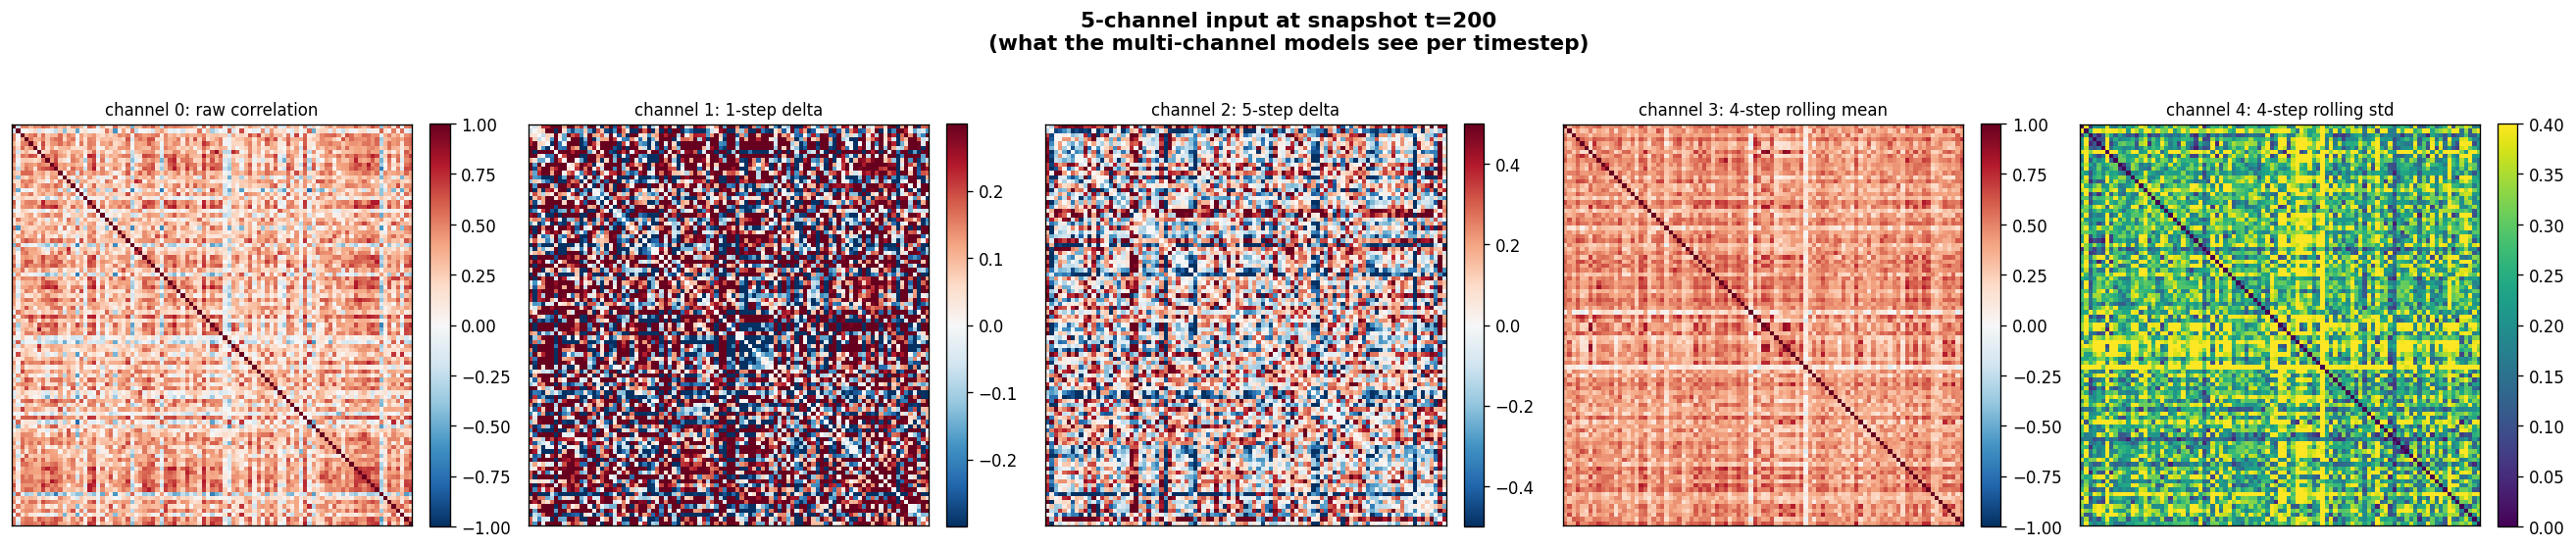
\includegraphics[width=\textwidth]{trial_channels_snapshot.png}
\caption{The five per-pixel channels for one snapshot: raw correlation,
one- and five-step change, and rolling mean and standard deviation. Each
gives the encoder a different view of the local temporal state of every
relationship.}
\label{fig:channels}
\end{figure}

\subsection{Stratified Volatility Split}\label{sec:split}

Standard temporal train/validation splits allocate all recent data
to validation. In our dataset, the period after April 2025 is
systematically less volatile than 2021--2024 (mean frame MSE 0.061
vs.\ 0.132). Under a naive temporal split, the validation set would
consist almost entirely of stable, easy-to-predict periods, while
the training set contains the volatile, hard periods. This creates
a systematic evaluation bias: models would be rewarded for learning
stable-period dynamics and penalized for volatile-period errors that
never appear in validation.

We resolve this with stratified volatility splitting. Snapshots with
$\text{MSE}_t$ above the median (volatile) and below the median
(stable) form separate strata, and within each stratum 70\% are
allocated to training and 30\% to validation. This ensures both
training and validation contain matched proportions of volatile
snapshots and span the full date range (2021--2026) rather than
concentrating the calm recent period in validation. The split yields
792 training and 340 validation snapshots. On this stratified
validation set the persistence baseline MSE is 0.128 and the
mean-frame baseline is 0.071 --- the latter being the harder bar to
beat, as it already captures the strong mean-reversion of correlations.

\subsection{Confidence-Conditioned Selective Prediction}
\label{sec:selective}

Aggregate directional accuracy, computed over all $N^2$ matrix cells,
treats every prediction equally. But the vast majority of the
predictable signal is concentrated in cells undergoing large coupling
changes, while small changes are dominated by noise that no model can
forecast (Sec.~\ref{sec:res_magnitude}). The aggregate metric therefore
\emph{dilutes} the model's genuine skill by averaging confident,
accurate predictions with unavoidable coin-flips on near-static pairs.

We make this skill usable with selective
prediction~\cite{geifman2017selective}. The model's
\emph{predicted change magnitude} for cell $(i,j)$,
$\hat{c}_{ij} = |\hat{R}^{(ij)}_{t+H} - R^{(ij)}_t|$, is available at
inference and serves as a confidence score. To predict at coverage
$q \in (0,1]$, we rank all cells by $\hat{c}_{ij}$ and emit directional
predictions only for the top-$q$ fraction, abstaining on the rest.
Sweeping $q$ traces a directional-accuracy-versus-coverage curve that
exposes the accuracy the model can deliver when permitted to abstain on
its low-confidence cells. As we show, this confidence score is
well-calibrated: predicted and realized change magnitudes correlate at
$0.47$, so the cells the model is most confident about are genuinely the
ones it predicts most accurately.

\subsection{Cross-Stock Inference via the Forecast}
\label{sec:crossstock}

A correlation forecast is ultimately useful if it improves inference
about asset returns. We test this directly: given the realized return
$r_B$ of one asset over the prediction window, the forecasted coupling
implies an estimate of a peer's return,
\begin{equation}
    \hat{r}_A = \hat{\rho}_{AB}\,\frac{\sigma_A}{\sigma_B}\, r_B,
\end{equation}
where $\sigma_A,\sigma_B$ are trailing volatilities. This is the
conditional-expectation (regression) relationship implied by the
predicted correlation. It is an \emph{inference} task --- observe one
leg, infer the other (as in hedging, portfolio completion, or scenario
analysis) --- not an ex-nihilo forecast. We compare the forecasted
$\hat{\rho}$ against three baselines for $\rho$: persistence (last
observed correlation), the historical mean correlation, and the
realized future correlation (an oracle upper bound), measuring how well
each predicts the actual $r_A$.

\subsection{Model Architectures}\label{sec:architectures}

We evaluate a broad set of video architectures, all using the same
dataset, combined loss, and evaluation protocol to enable fair
comparison. We describe the three that anchor the study below;
EfficientNet transfer learning, PredRNN, and a factorized space-time
Transformer were also evaluated (Sec.~\ref{sec:res_ceiling}). ConvLSTM
emerged as the strongest single model once multi-channel inputs were
introduced and is used for all subsequent analysis.

\textbf{CNN+LSTM.} A 2D CNN encoder is applied independently to
each frame in the lookback sequence, extracting a 256-dimensional
spatial feature vector. Three convolutional layers with kernel sizes
5, 5, and 3 detect progressively larger spatial structures: the
first layer detects local pair-level correlation patterns (small
clusters, cluster edges), the second detects broader cluster blocks
and inter-cluster relationships, and the third refines fine-grained
patterns within clusters. Batch normalization and max-pooling
(stride 2) after each of the first two layers reduce the spatial
dimension from $95\times95$ to $\approx23\times23$ before adaptive
average pooling to a fixed $6\times6$ output. An LSTM with 256
hidden units and 2 layers then processes the sequence of 20 frame
encodings, with the final hidden state decoded to the predicted
$95\times95$ matrix via a three-layer MLP with Tanh output to
constrain predictions to $[-1, +1]$.

The key limitation of this architecture is that spatial structure is
discarded after the CNN encoder: the LSTM operates on 256-dimensional
vectors, not on spatial feature maps. Temporal reasoning happens on
abstract features rather than on the raw spatial structure of the
correlation matrix.

\textbf{3D CNN.} 3D convolutional kernels operate simultaneously
over spatial and temporal dimensions of the input volume
$(L, N, N) = (20, 95, 95)$, treating it as a 3D tensor with a
single channel. A kernel of size $(T_k, H_k, W_k)$ detects the
same spatial pattern changing over $T_k$ consecutive frames ---
for example, a $(3,3,3)$ kernel can detect ``this 3-stock cluster
has been brightening over the past 3 days.'' This is more direct
than CNN+LSTM because temporal context is captured at the level
of spatial pixels rather than at the level of compressed feature
vectors.

Four convolutional blocks use kernels of sizes $(3,3,3)$, $(3,5,5)$,
$(5,3,3)$, and $(3,3,3)$ to capture short-range spatiotemporal
patterns, broader spatial context, longer temporal patterns, and
deep features respectively. The batch size was reduced to 8 due to
higher GPU memory requirements (approximately 4.5GB per forward
pass on the $(8, 1, 20, 95, 95)$ input tensor).

\textbf{ConvLSTM~\cite{shi2015convolutional}.} Addresses the
spatial discarding problem of CNN+LSTM by maintaining spatial
feature maps as the hidden state throughout temporal processing.
At each timestep $t$, the ConvLSTM cell takes a spatial feature
map $\mathbf{x}_t \in \mathbb{R}^{C \times H \times W}$ and updates
spatial hidden and cell states $\mathbf{h}_t, \mathbf{c}_t \in
\mathbb{R}^{C' \times H \times W}$ via convolutional gates:
\begin{align}
    \mathbf{i}_t &= \sigma(\mathbf{W}_{xi} \ast \mathbf{x}_t +
                    \mathbf{W}_{hi} \ast \mathbf{h}_{t-1}) \\
    \mathbf{f}_t &= \sigma(\mathbf{W}_{xf} \ast \mathbf{x}_t +
                    \mathbf{W}_{hf} \ast \mathbf{h}_{t-1}) \\
    \mathbf{c}_t &= \mathbf{f}_t \odot \mathbf{c}_{t-1} +
                    \mathbf{i}_t \odot \tanh(\mathbf{W}_{xc}
                    \ast \mathbf{x}_t + \mathbf{W}_{hc}
                    \ast \mathbf{h}_{t-1}) \\
    \mathbf{h}_t &= \mathbf{o}_t \odot \tanh(\mathbf{c}_t)
\end{align}
where $\ast$ denotes convolution and $\odot$ element-wise product.
The spatial hidden state allows the model to track how specific
regions of the correlation matrix (specific asset pairs and clusters)
evolve over time without compressing spatial information to vectors.
Frames are first downsampled from $95\times95$ to $24\times24$ via
a convolutional encoder to reduce memory requirements.

\textbf{PredRNN and space-time Transformer.} To test whether more
expressive temporal modeling breaks the ceiling, we additionally
evaluate PredRNN~\cite{wang2017predrnn}, whose spatiotemporal LSTM
cells propagate a memory state both across time and up through layers,
and a factorized space-time Transformer in the style of
TimeSformer~\cite{bertasius2021space}, which patch-tokenizes each frame
and applies spatial self-attention within frames followed by temporal
self-attention across frames. An EfficientNet-B0~\cite{tan2019efficientnet}
transfer-learning encoder was also evaluated. None of these surpasses
ConvLSTM (Sec.~\ref{sec:res_ceiling}), reinforcing that the ceiling is
a property of the data rather than of model capacity.

All models share the same decoder: a three-layer MLP
($d_{\text{hidden}} \to 1024 \to 2048 \to N^2$) with ReLU activations
and Tanh output that maps the final spatial/recurrent representation to
the predicted $N \times N = 95 \times 95 = 9025$ correlation values.
% ══════════════════════════════════════════════════════════════════════════════
\section{Experiments}\label{sec:experiments}
% ══════════════════════════════════════════════════════════════════════════════

\subsection{Dataset}

We use 5-minute bar data for 95 Nifty 100 constituent stocks from
July 30, 2021 to April 8, 2026, comprising 87,122 aligned timesteps.
EWMA correlations ($\lambda=0.94$) are computed for all 4,465 pairs.
Daily correlation matrix snapshots are built at every 75-bar interval,
yielding 1,157 snapshots. The Fiedler vector naturally separates
defensive/consumer stocks (FMCG, pharmaceuticals) from cyclical/growth
stocks at the extremes.

\textbf{Split.} Stratified by volatility (Sec.~\ref{sec:split}):
792 training and 340 validation snapshots, with matched volatile
proportions and full date-range coverage in both.

\subsection{Baselines}

\textbf{Persistence.} Predicts $\hat{R}_{t+H} = R_t$. MSE = 0.128.

\textbf{Mean-frame.} Predicts $\hat{R}_{t+H} = \bar{R}_{\text{train}}$.
MSE = 0.071. This captures the strong mean-reversion tendency of
correlations and is the harder baseline to beat.

\subsection{Evaluation Metrics}

\textbf{MSE (unweighted).} Mean squared error between predicted and
actual matrices.

\textbf{Pearson $r$.} Correlation between all predicted and actual
values, measuring structural agreement beyond MSE.

\textbf{Directional accuracy.} Fraction of pairs where predicted
direction of correlation change matches actual direction.

\textbf{MSE on volatile/stable snapshots.} Separate MSE for snapshots
above and below the volatility threshold.

\subsection{Implementation Details}

All models use the Adam optimizer (learning rate $10^{-3}$, weight
decay $10^{-4}$), gradient clipping at 1.0, cosine annealing with warm
restarts ($T_0=20$, $T_{\text{mult}}=2$), and early stopping with
patience 15. Inputs use a 20-snapshot lookback with the five-channel
representation of Sec.~\ref{sec:channels}. Training is on an NVIDIA
RTX 4070 Laptop GPU (8GB VRAM) with batch size 16.

% ══════════════════════════════════════════════════════════════════════════════
\section{Results}\label{sec:results}
% ══════════════════════════════════════════════════════════════════════════════

\subsection{Correlation Matrix Video Quality}

Fig.~\ref{fig:frames} shows sample frames of the Fiedler-ordered
correlation matrix video. Diagonal block structure is clearly visible
and varies substantially across market regimes, confirming that the
ordering produces spatially coherent cluster patterns suitable for
convolutional processing.

\begin{figure}[H]
\centering
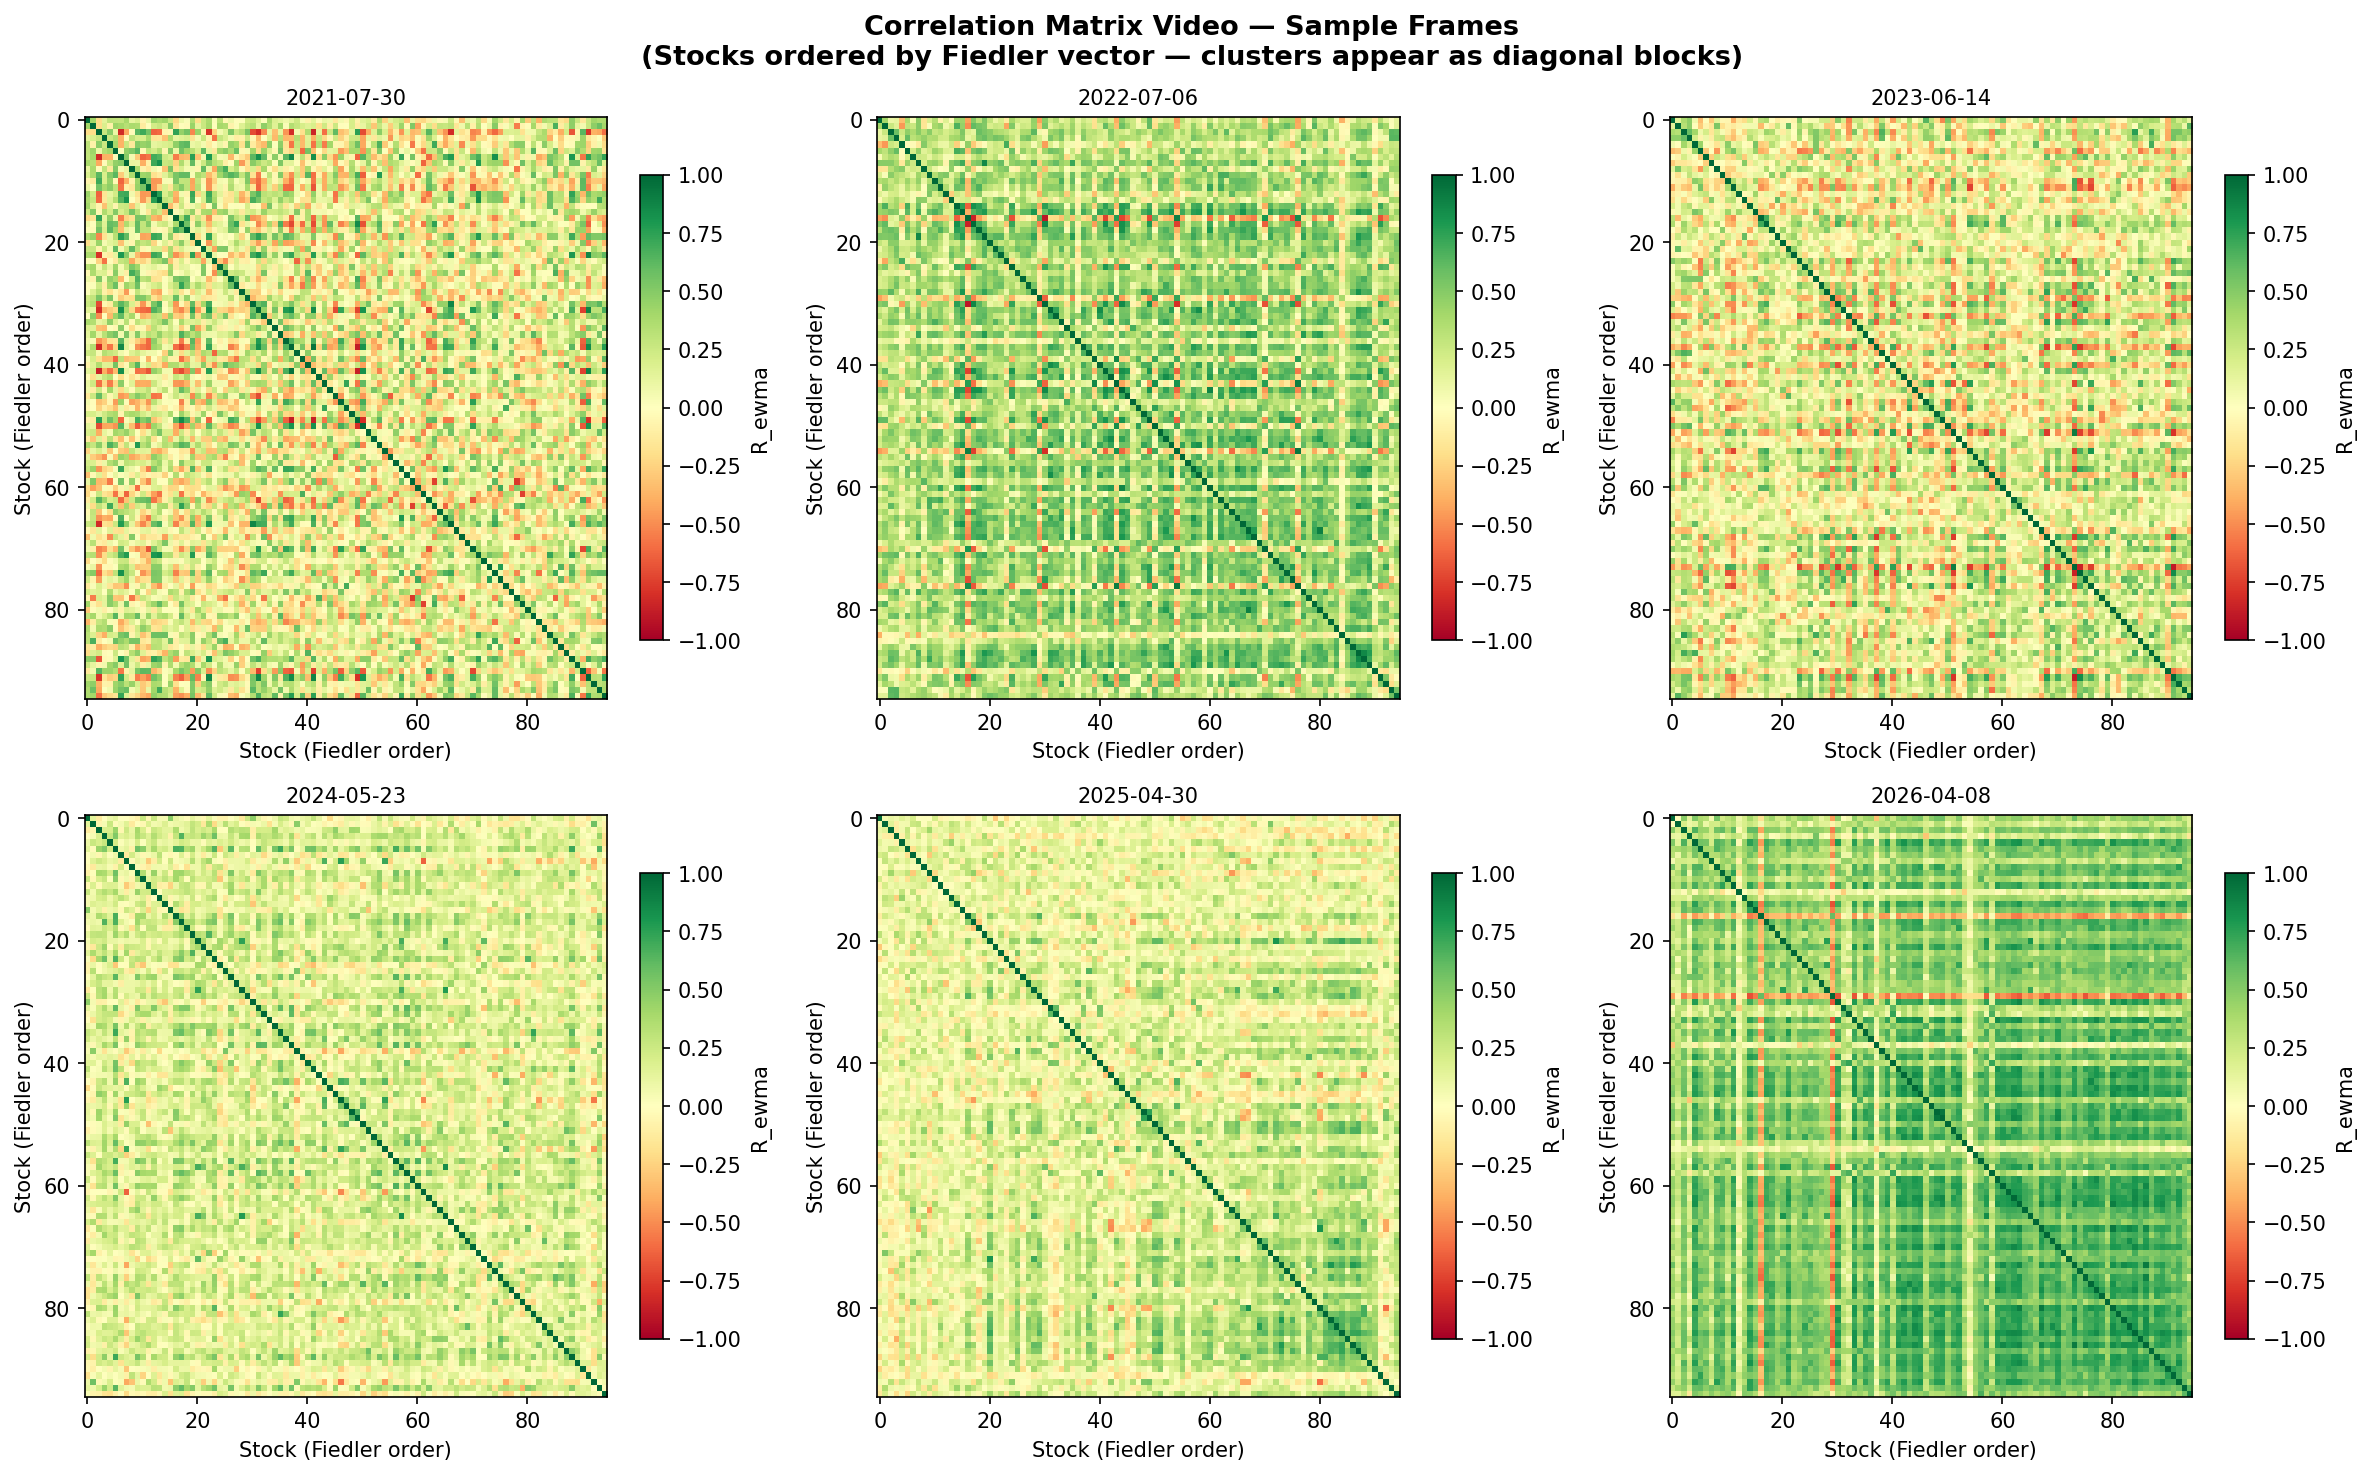
\includegraphics[width=\textwidth]{plot_cell11_corr_frames.png}
\caption{Sample frames of the Fiedler-ordered correlation matrix video.
Green indicates strong positive correlation; red indicates negative
correlation. Visible diagonal block structure confirms spatially
coherent cluster patterns.}
\label{fig:frames}
\end{figure}

That the pixels carry genuine financial signal is confirmed in
Fig.~\ref{fig:pixel_intensity}: a same-sector pair (HDFCBANK--ICICIBANK)
exhibits consistently high coupling, while a cross-sector pair
(RELIANCE--INFY) is lower and more variable. Fig.~\ref{fig:framestats}
shows the market-wide mean and dispersion of coupling over time, making
regime shifts --- periods where the whole market couples --- directly
visible as a video-level brightness signal.

\begin{figure}[H]
\centering
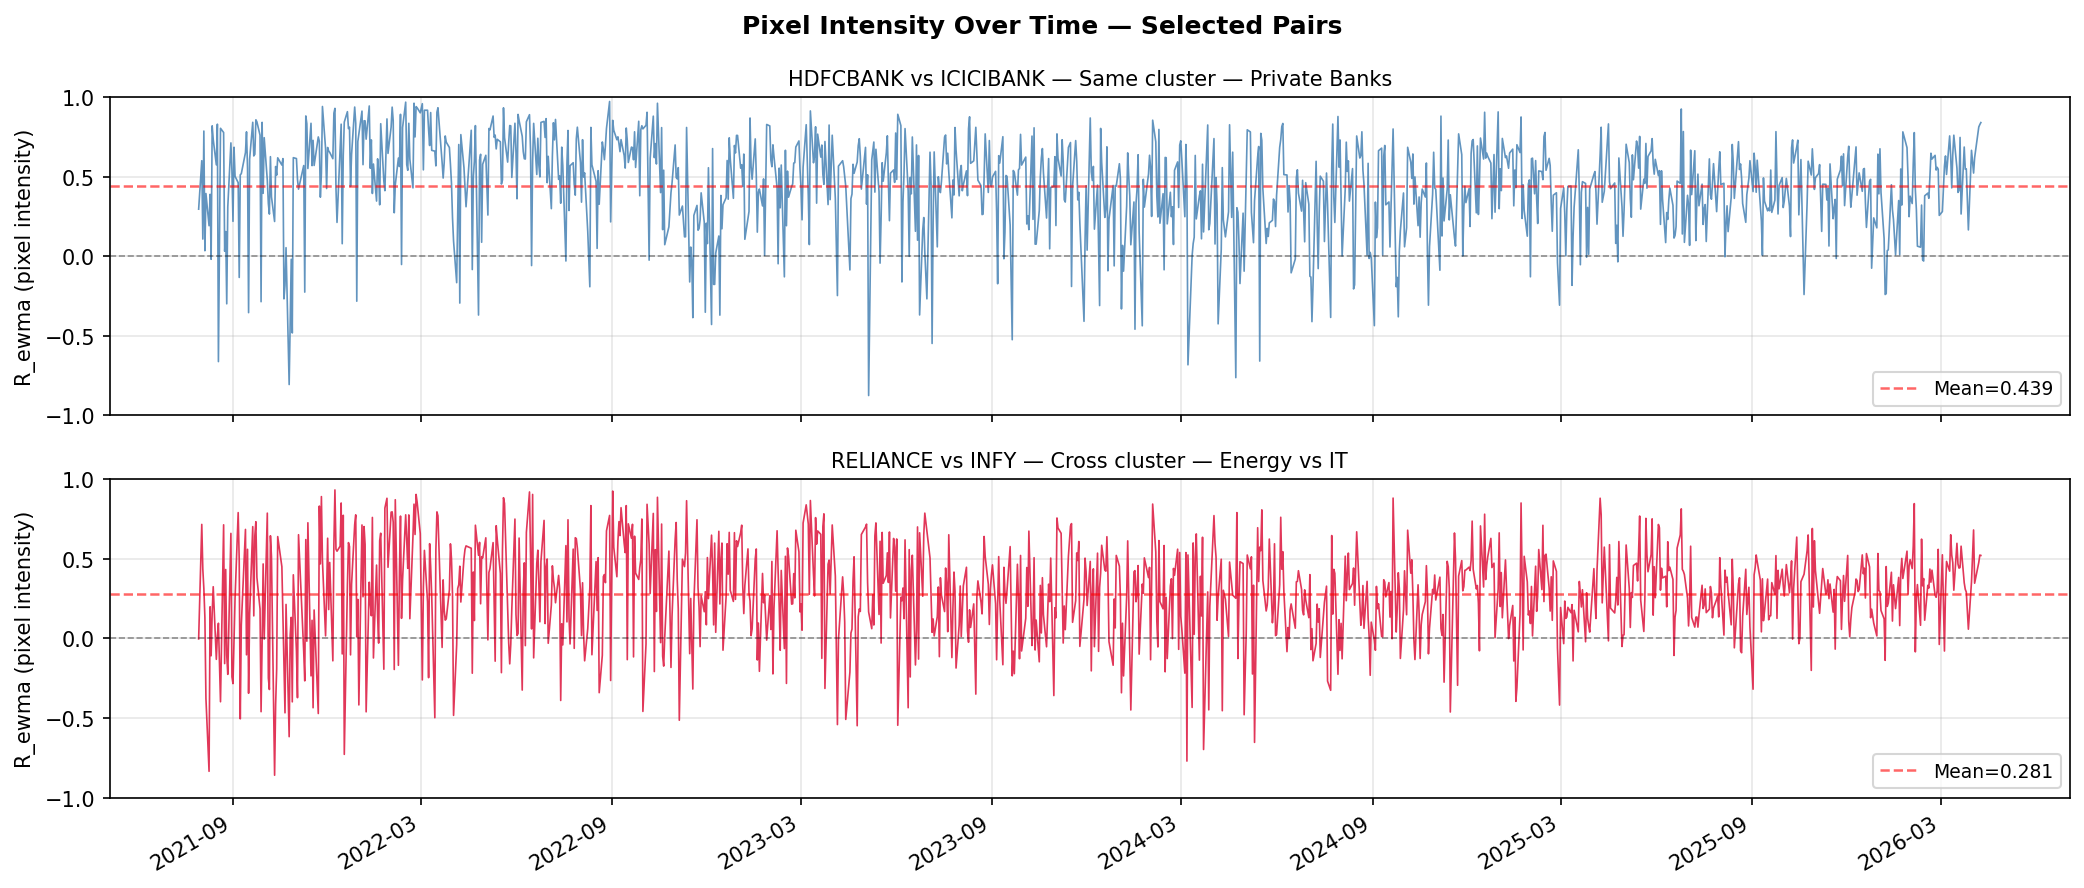
\includegraphics[width=\textwidth]{plot_cell11_pixel_intensity.png}
\caption{Pixel intensity (EWMA correlation) over time for two asset
pairs. The same-sector pair stays bright; the cross-sector pair is
dimmer and more variable, confirming that pixel values carry meaningful
financial signal.}
\label{fig:pixel_intensity}
\end{figure}

\begin{figure}[H]
\centering
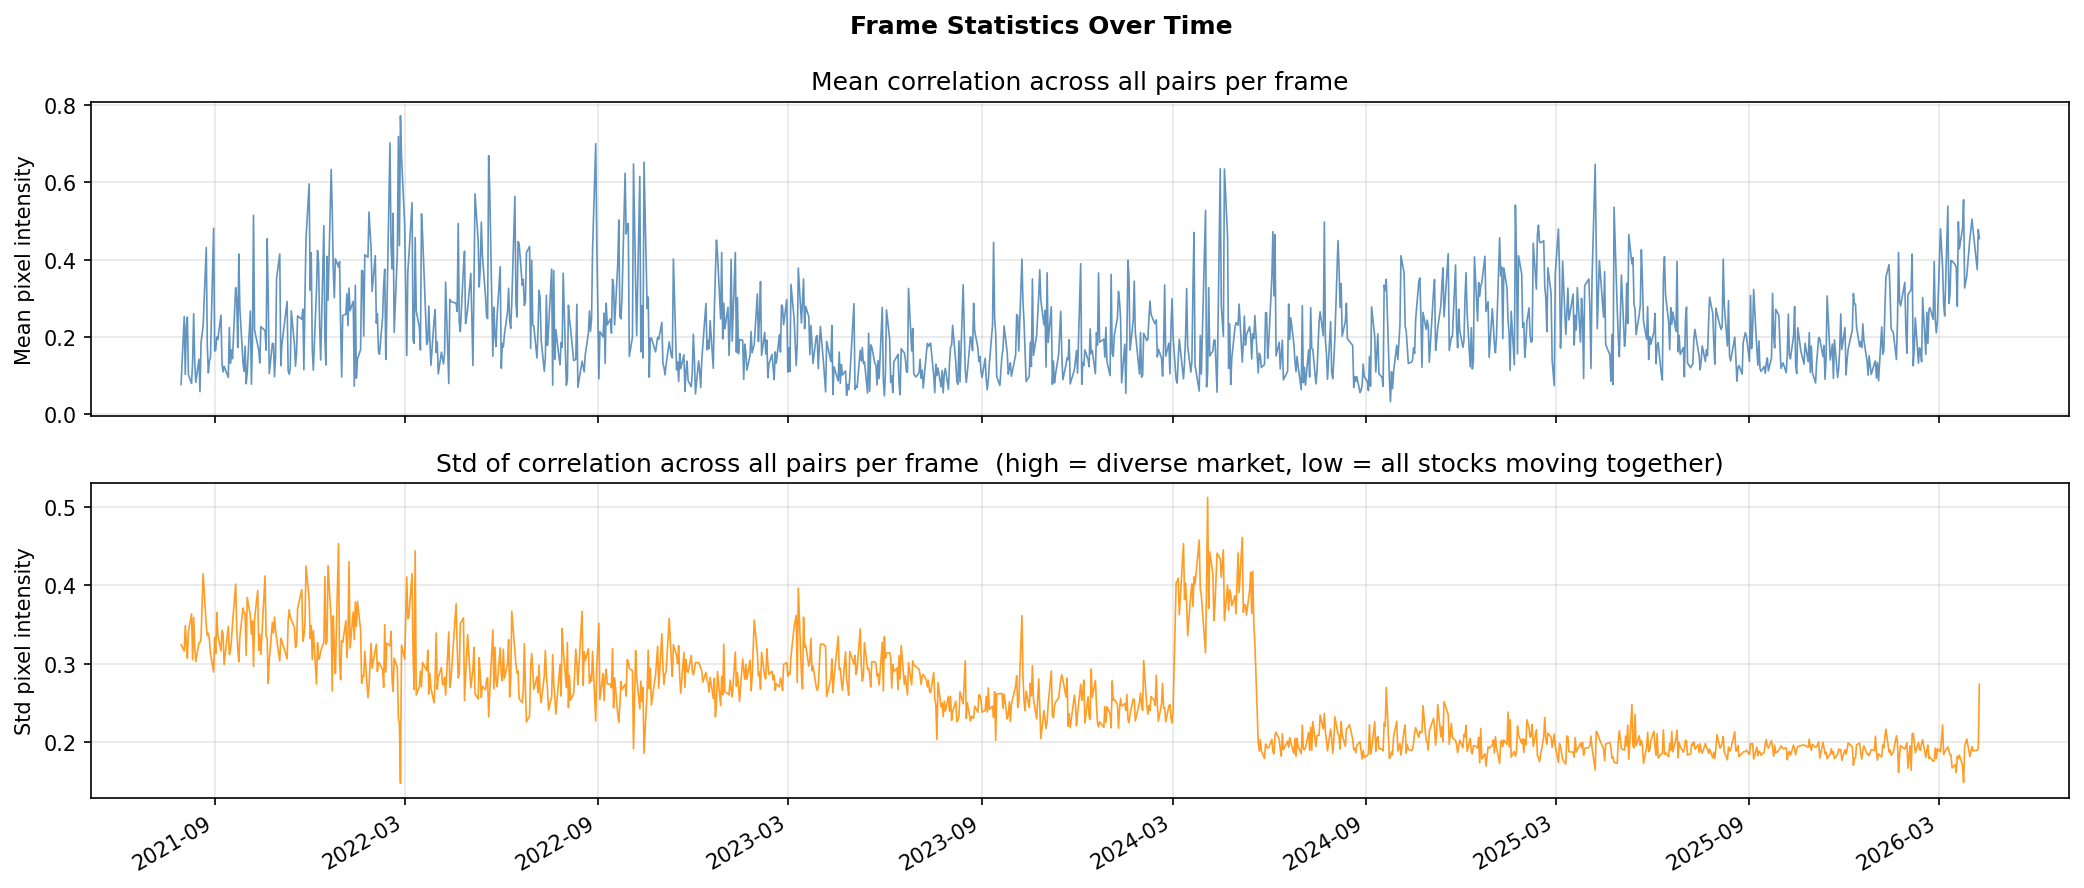
\includegraphics[width=\textwidth]{plot_cell11_frame_stats.png}
\caption{Frame-level statistics over time: mean coupling (top) and
cross-sectional dispersion (bottom). High mean with low dispersion marks
market-wide co-movement regimes; the reverse marks idiosyncratic,
well-diversified periods.}
\label{fig:framestats}
\end{figure}

\subsection{A Shared Ceiling Across Architectures and Modalities}
\label{sec:res_ceiling}

Table~\ref{tab:ceiling} reports the best model under each architecture
and input modality. The striking result is convergence: every
configuration --- four architecture families, plus volume- and
volatility-correlation input modalities --- lands at MSE $\approx 0.069$
and directional accuracy $\approx 73\%$. PredRNN's spatiotemporal memory
and the Transformer's global attention do not surpass ConvLSTM; adding
volume correlation is neutral and volatility correlation is mildly
harmful (the latter is a near-global factor that dilutes the per-pair
signal). The inter-architecture spread (0.0686--0.0721) is comparable to
the inter-seed variance we observe on a fixed architecture, indicating
that the ceiling is a property of the prediction problem, not of model
capacity or input modality.

\begin{table}[H]
\caption{Best configuration per architecture and input modality on the
stratified validation set. All converge to MSE $\approx0.069$,
directional accuracy $\approx73\%$. Combined loss; multi-channel inputs.}
\label{tab:ceiling}
\centering
\begin{tabular}{lccc}
\toprule
\textbf{Configuration} &
\textbf{MSE}$\downarrow$ &
\textbf{Pearson $r$}$\uparrow$ &
\textbf{Dir.\ Acc.}$\uparrow$ \\
\midrule
Persistence baseline          & 0.128 & ---   & 50.0\% \\
Mean-frame baseline           & 0.071 & ---   & ---    \\
\midrule
CNN+LSTM                      & \textbf{0.0681} & \textbf{0.387} & 0.732 \\
3D CNN                        & 0.0683 & 0.376 & \textbf{0.733} \\
ConvLSTM                      & 0.0686 & 0.372 & 0.730 \\
PredRNN                       & 0.0721 & 0.295 & 0.724 \\
Space-time Transformer        & 0.0712 & 0.317 & 0.726 \\
\midrule
ConvLSTM + volume corr.       & 0.0697 & 0.360 & 0.729 \\
ConvLSTM + volatility corr.   & 0.0721 & 0.293 & 0.723 \\
\bottomrule
\end{tabular}
\end{table}

\begin{figure}[H]
\centering
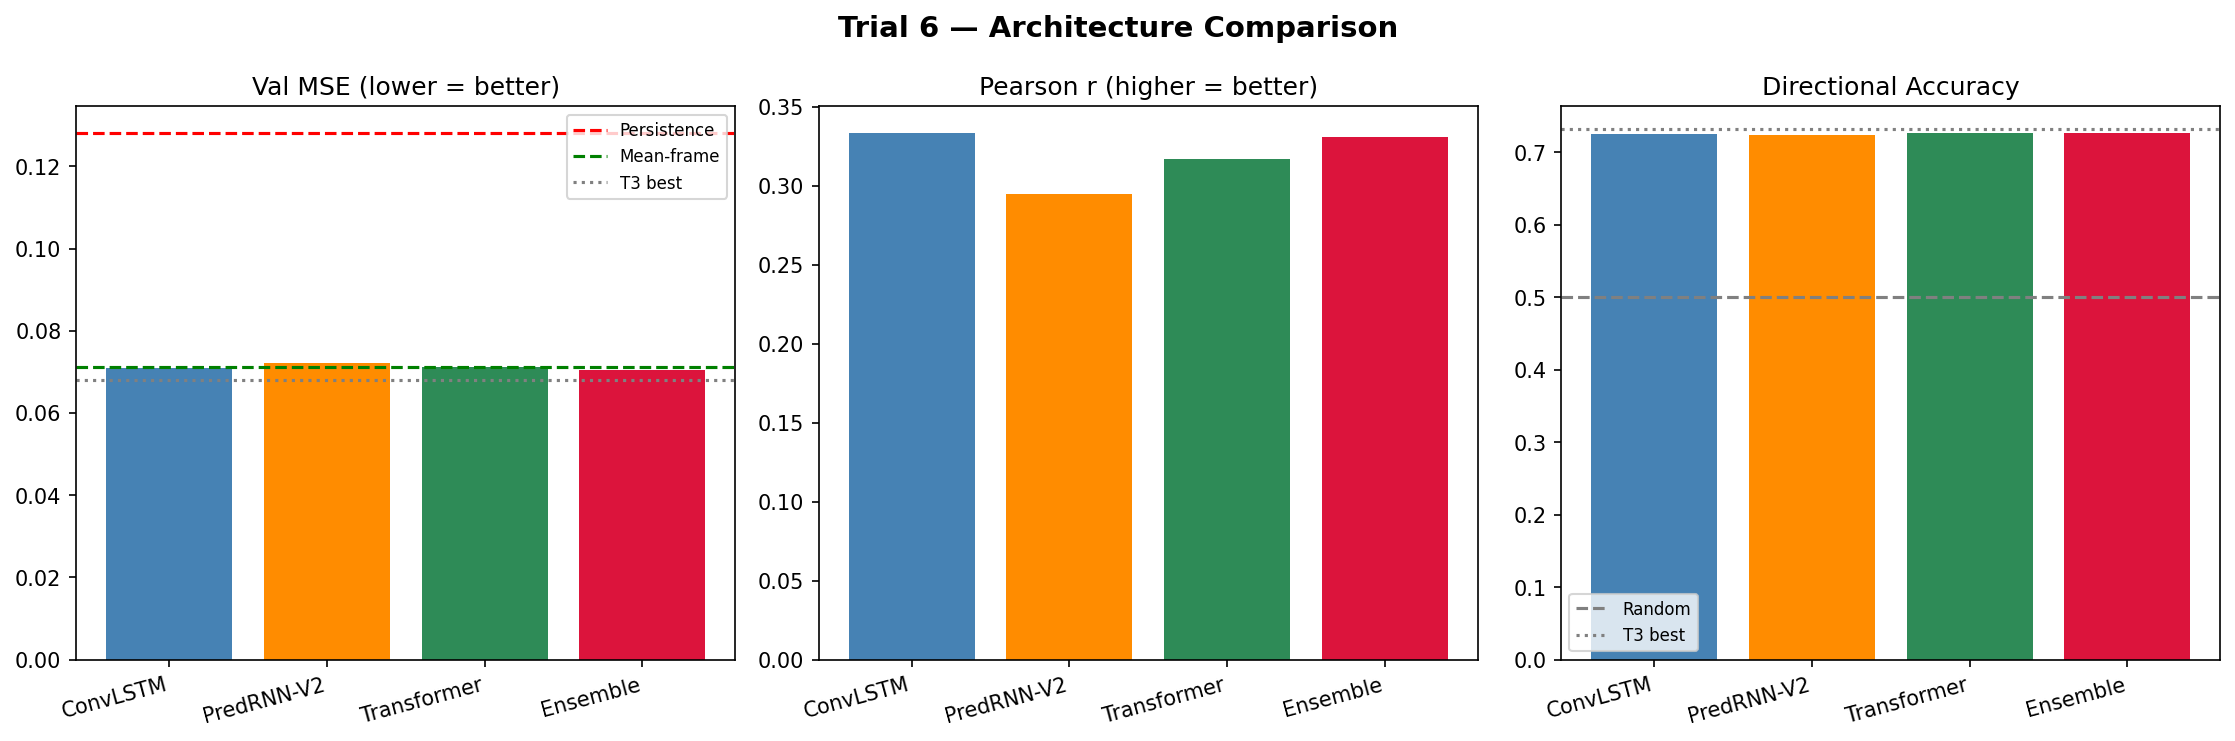
\includegraphics[width=\textwidth]{trial6_comparison.png}
\caption{Architecture comparison (ConvLSTM, PredRNN, space-time
Transformer, ensemble). All cluster at MSE $\approx0.07$ and
directional accuracy $\approx0.73$, illustrating the shared ceiling.}
\label{fig:arch}
\end{figure}

The input-modality result deserves emphasis because the volume and
volatility channels are \emph{not} redundant with returns:
Fig.~\ref{fig:volsig} shows that, across representative pairs, rolling
volume- and volatility-correlation carry information largely independent
of return-correlation (average cross-stream correlations of 0.18 and
0.25). Fig.~\ref{fig:threevideos} visualizes the three modality videos
side by side --- they exhibit visibly different block structure.
Despite this genuine independence, adding them as input channels does
not help: the modality ablation ladder (Fig.~\ref{fig:modality}) shows
volume neutral and volatility mildly harmful relative to the
return-only baseline. Independent information is not the same as
\emph{predictive} information for this target.

\begin{figure}[H]
\centering
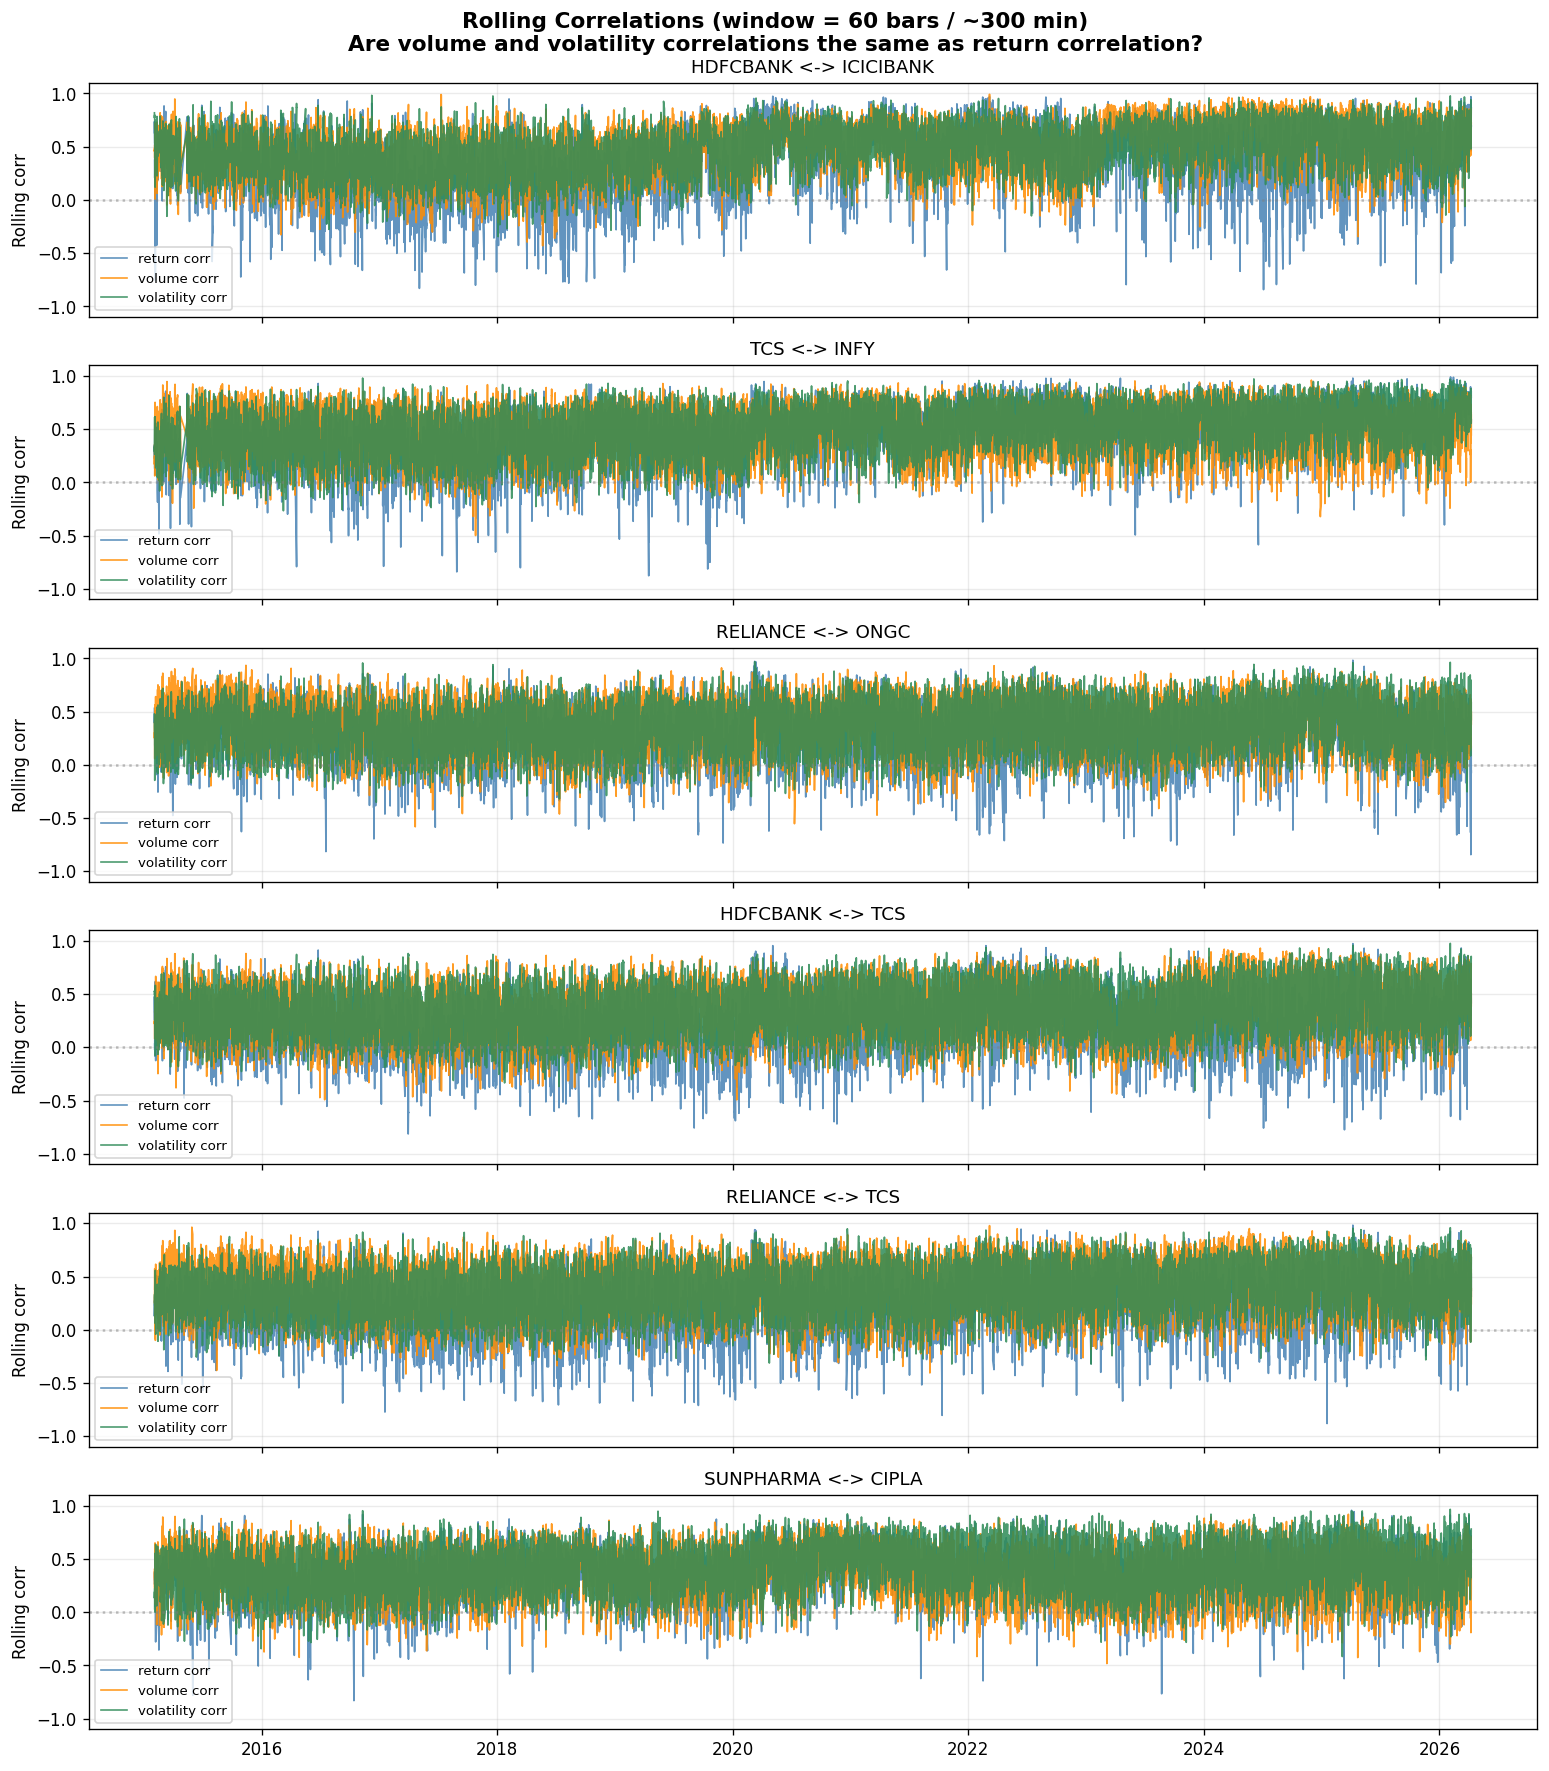
\includegraphics[width=\textwidth]{volume_signal_check.png}
\caption{Rolling return-, volume-, and volatility-correlation for
representative pairs. Volume and volatility coupling move largely
independently of return coupling, confirming they are distinct signals.}
\label{fig:volsig}
\end{figure}

\begin{figure}[H]
\centering
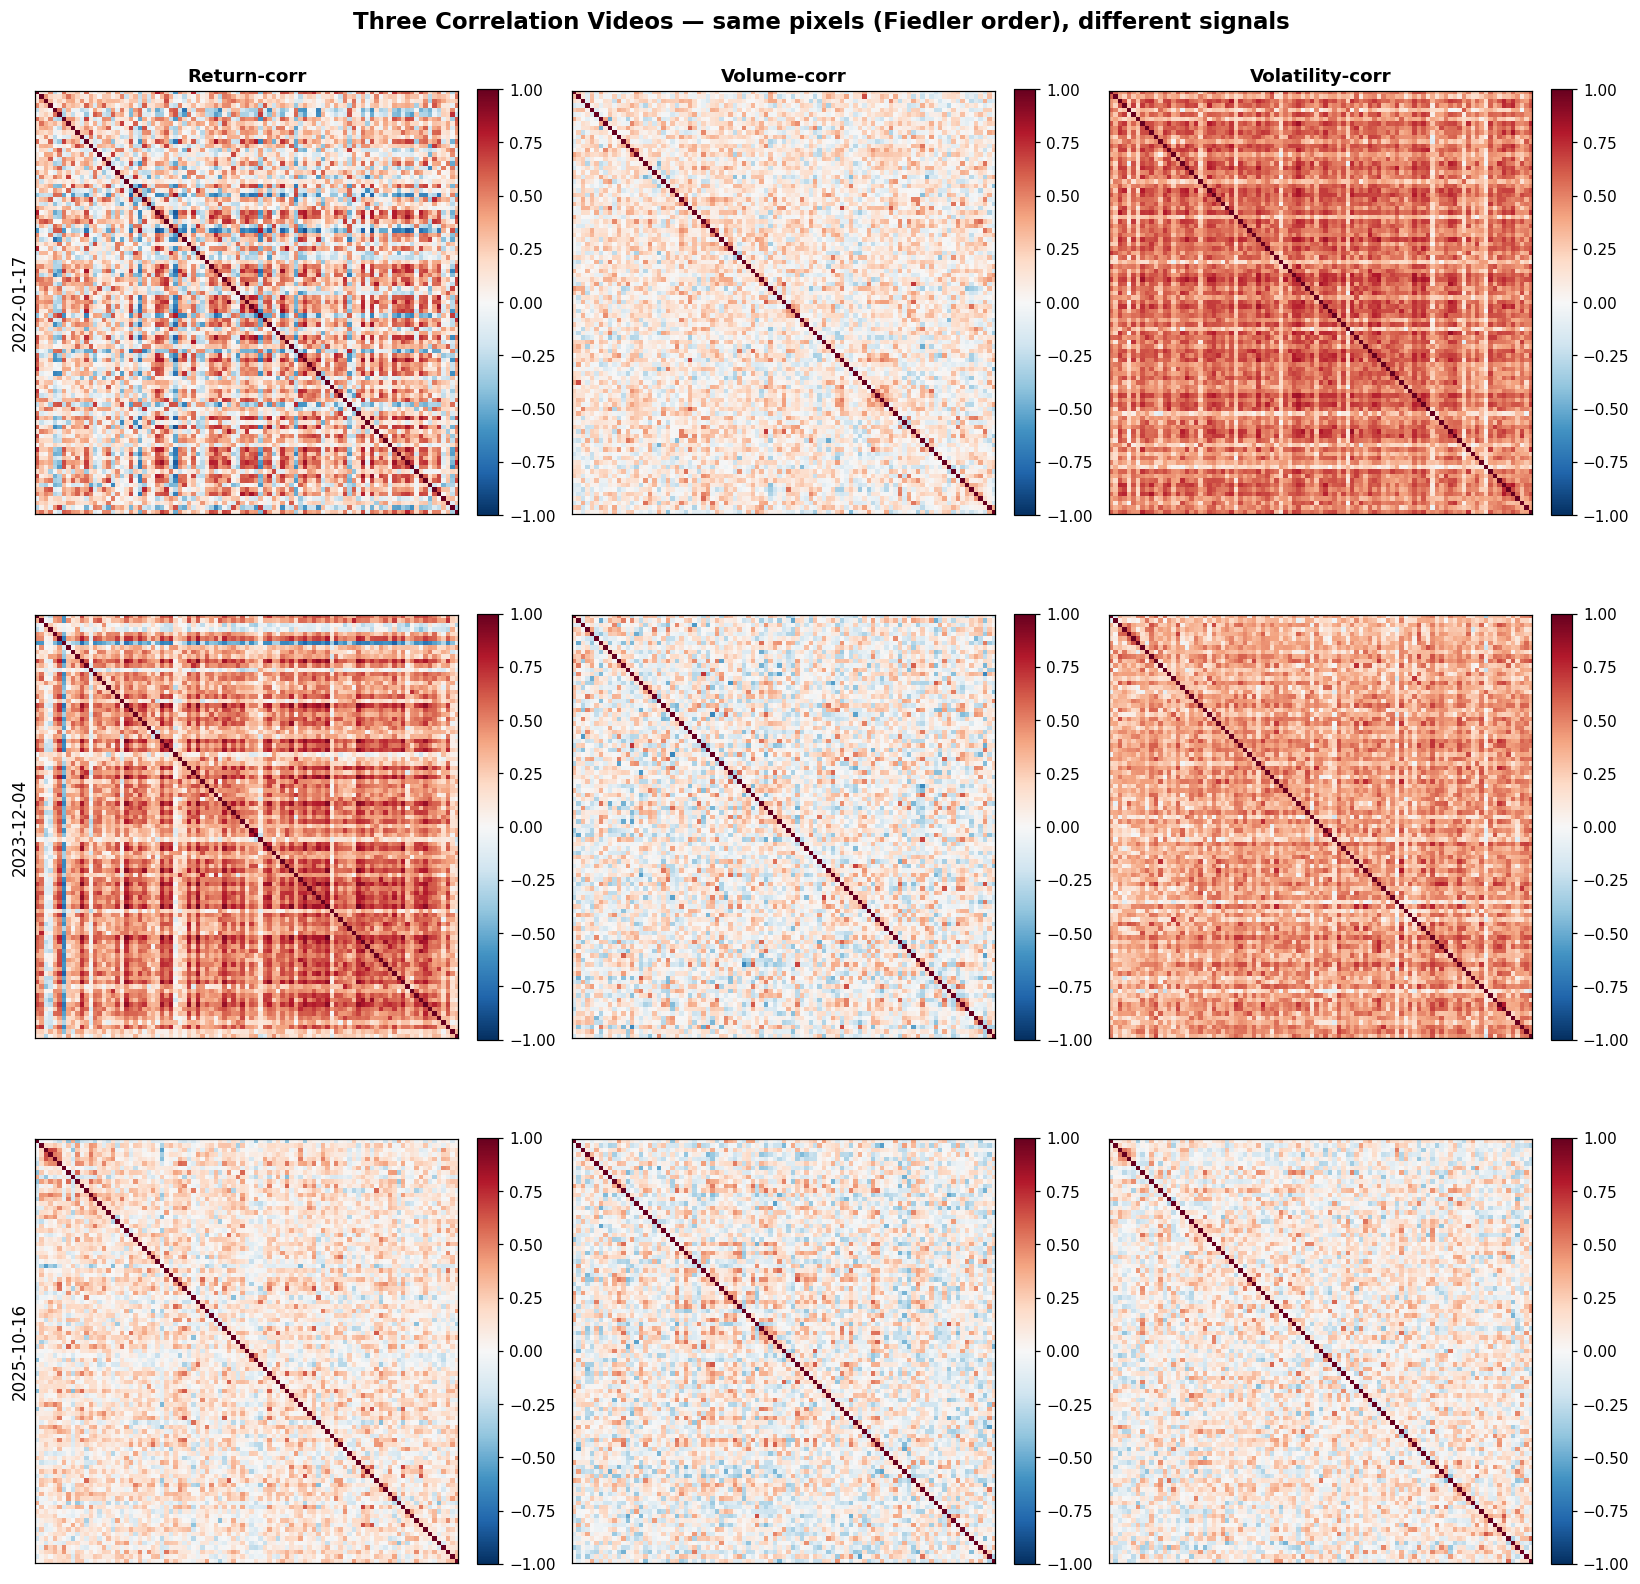
\includegraphics[width=\textwidth]{three_videos_compare.png}
\caption{The three correlation-video modalities at matched snapshots
(identical Fiedler layout): return (left), volume (center), volatility
(right). The distinct block patterns confirm independent structure;
the per-frame cross-correlations are low.}
\label{fig:threevideos}
\end{figure}

\begin{figure}[H]
\centering
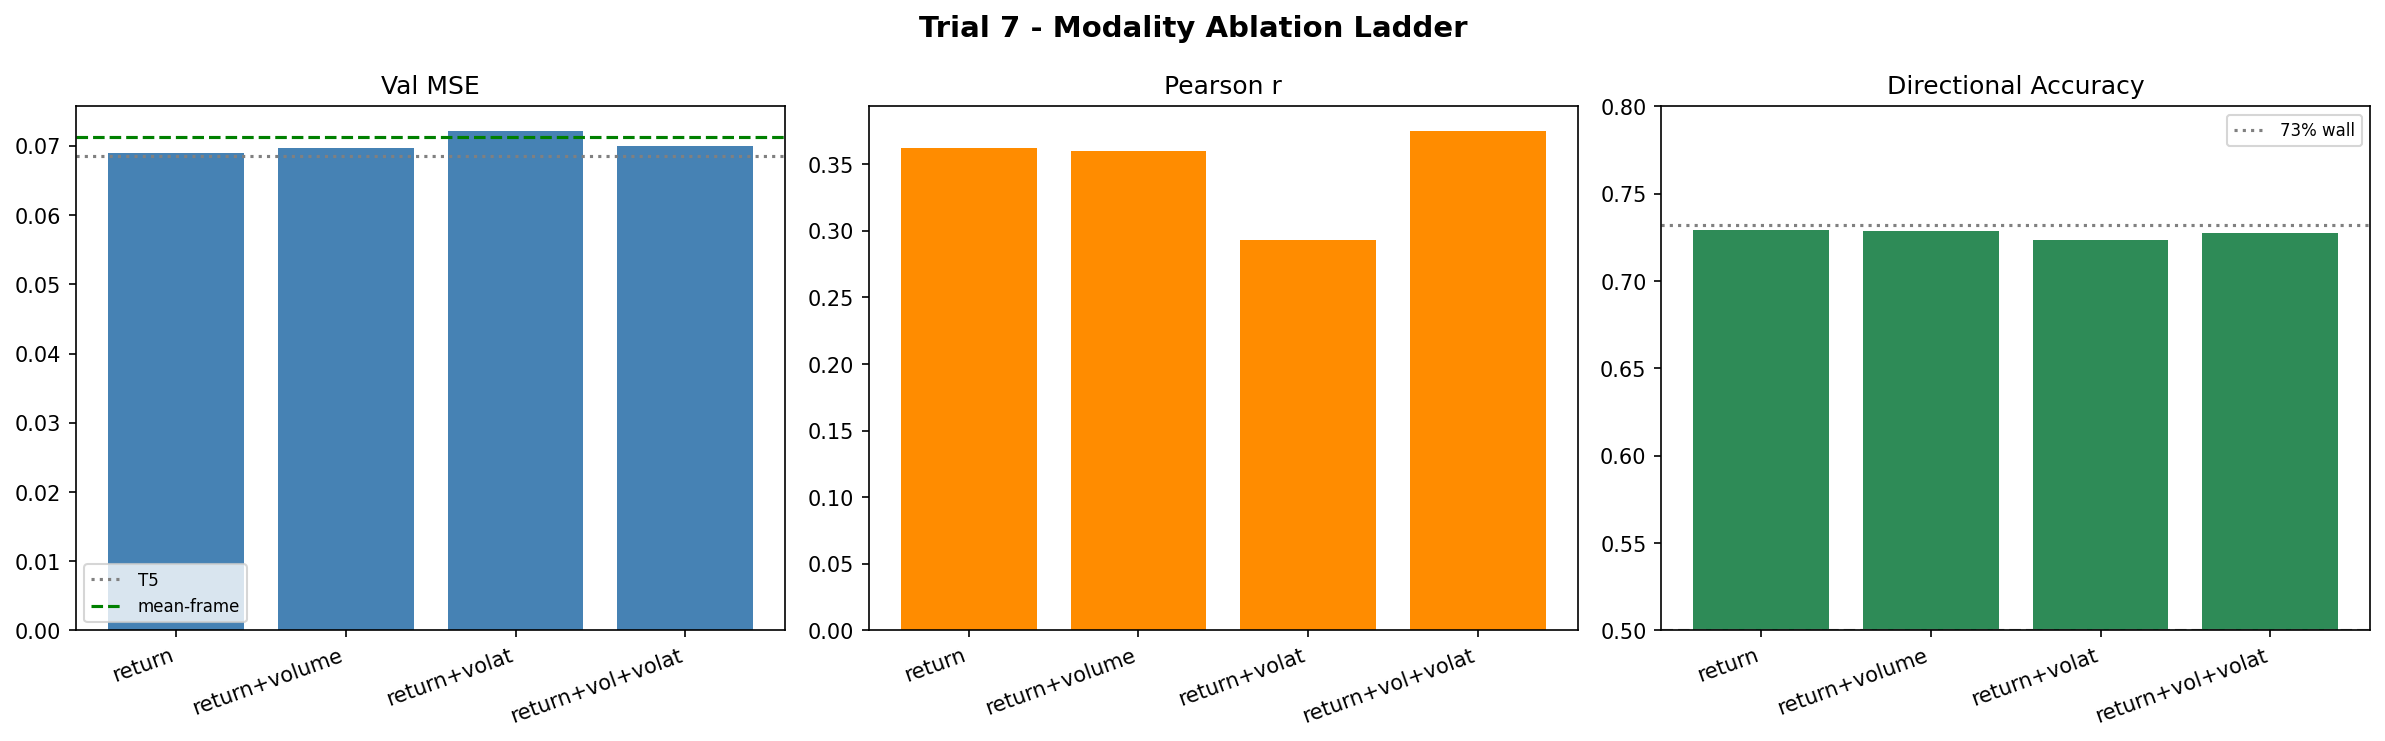
\includegraphics[width=\textwidth]{trial7_ablation.png}
\caption{Modality ablation ladder: ConvLSTM trained on return only,
return$+$volume, return$+$volatility, and all three. No modality beats
the return-only baseline; volatility correlation degrades it.}
\label{fig:modality}
\end{figure}

\subsection{Predictability Rises with Change Magnitude}
\label{sec:res_magnitude}

The aggregate 73\% obscures strong structure. Table~\ref{tab:magnitude}
stratifies directional predictability by the magnitude of the actual
correlation change: it rises monotonically from 73\% over all pairs to
88\% on changes exceeding 0.30. A one-line mean-reversion rule (predict
that coupling reverts toward its 20-snapshot mean) already attains 73\%
over all pairs --- matching the deep models --- and the same rule reaches
88\% on the largest moves. The implication is twofold: (i) most of the
deep model's aggregate skill coincides with mean-reversion, and (ii) the
genuinely predictable signal lives in the large-magnitude changes, which
the aggregate metric averages away.

\begin{table}[H]
\caption{Best directional accuracy stratified by magnitude of the true
correlation change. Predictability rises sharply with magnitude.}
\label{tab:magnitude}
\centering
\begin{tabular}{lcc}
\toprule
\textbf{Change magnitude} & \textbf{\% of cells} & \textbf{Dir.\ Acc.} \\
\midrule
all cells          & 100.0\% & 0.734 \\
$> 0.10$           & 76.2\%  & 0.790 \\
$> 0.15$           & 65.1\%  & 0.816 \\
$> 0.20$           & 54.9\%  & 0.841 \\
$> 0.30$           & 37.5\%  & 0.884 \\
\bottomrule
\end{tabular}
\end{table}

\begin{figure}[H]
\centering
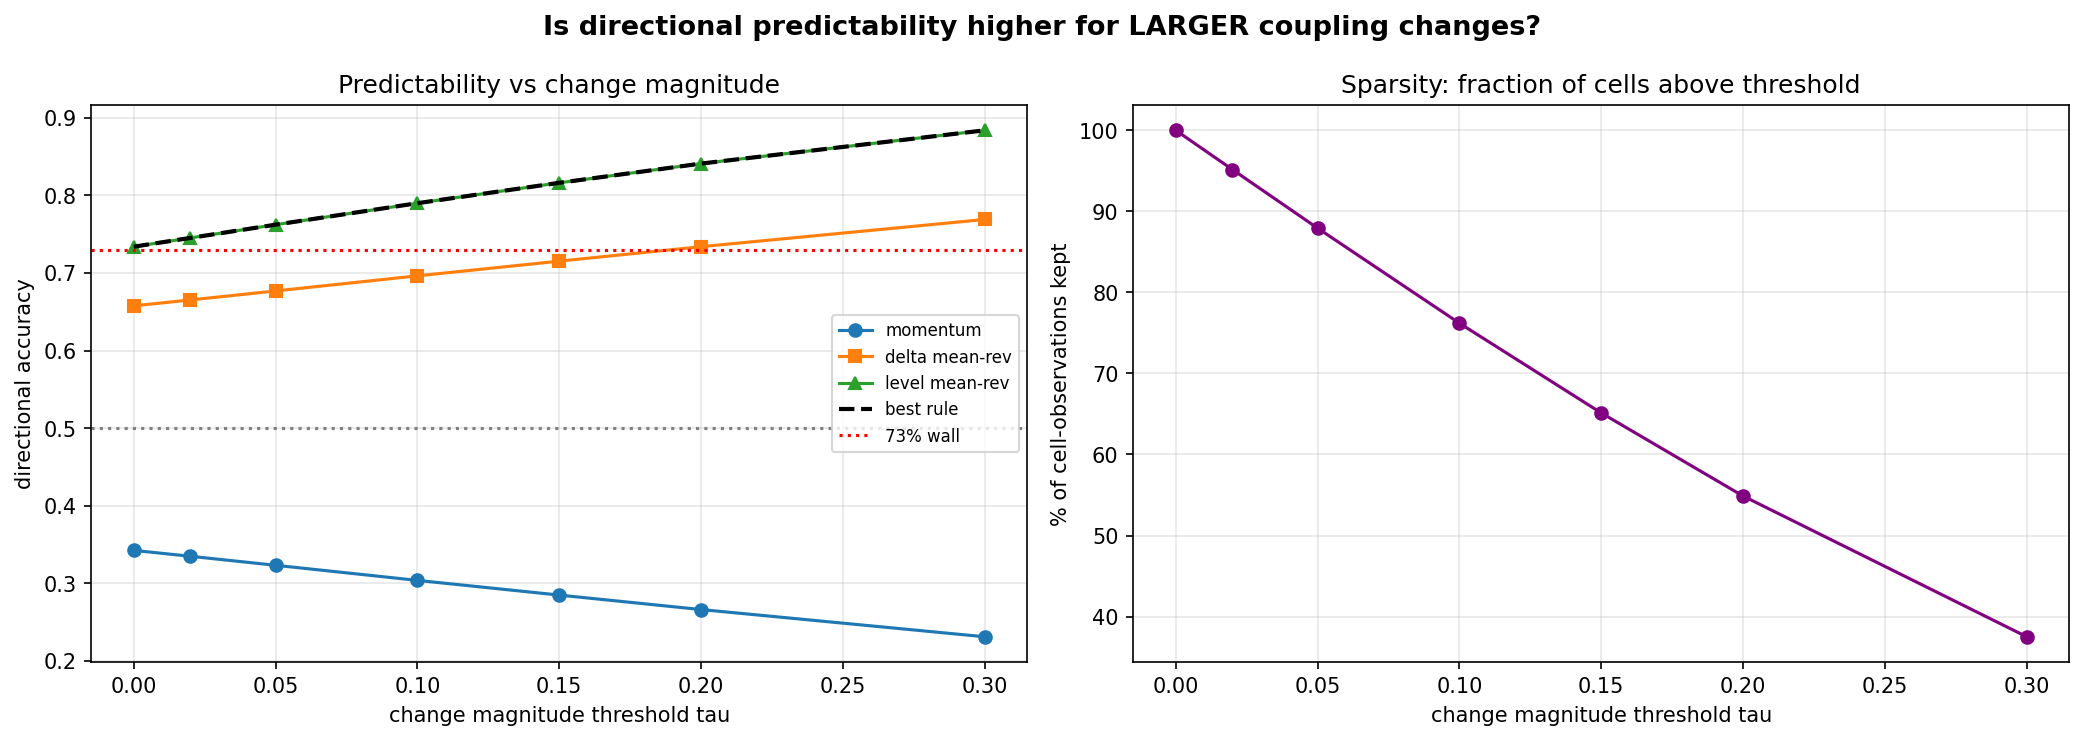
\includegraphics[width=\textwidth]{magnitude_ablation.png}
\caption{Directional predictability versus change-magnitude threshold
(left) and the corresponding fraction of cells retained (right).
Predictability rises steeply with magnitude; the dashed line marks the
73\% aggregate.}
\label{fig:magnitude}
\end{figure}

We stress that this is \emph{not} a sparse-event regime: large changes
are common (the median five-day coupling change is 0.23), and they do
not concentrate on a fixed subset of ``event-prone'' pairs ---
Fig.~\ref{fig:eventstruct} shows the per-pair frequency of large moves
is nearly uniform and only weakly persistent over time. There is thus no
static watchlist to exploit; the structure to exploit is the
\emph{magnitude} of each predicted change, which motivates the
confidence-conditioned approach below.

\begin{figure}[H]
\centering
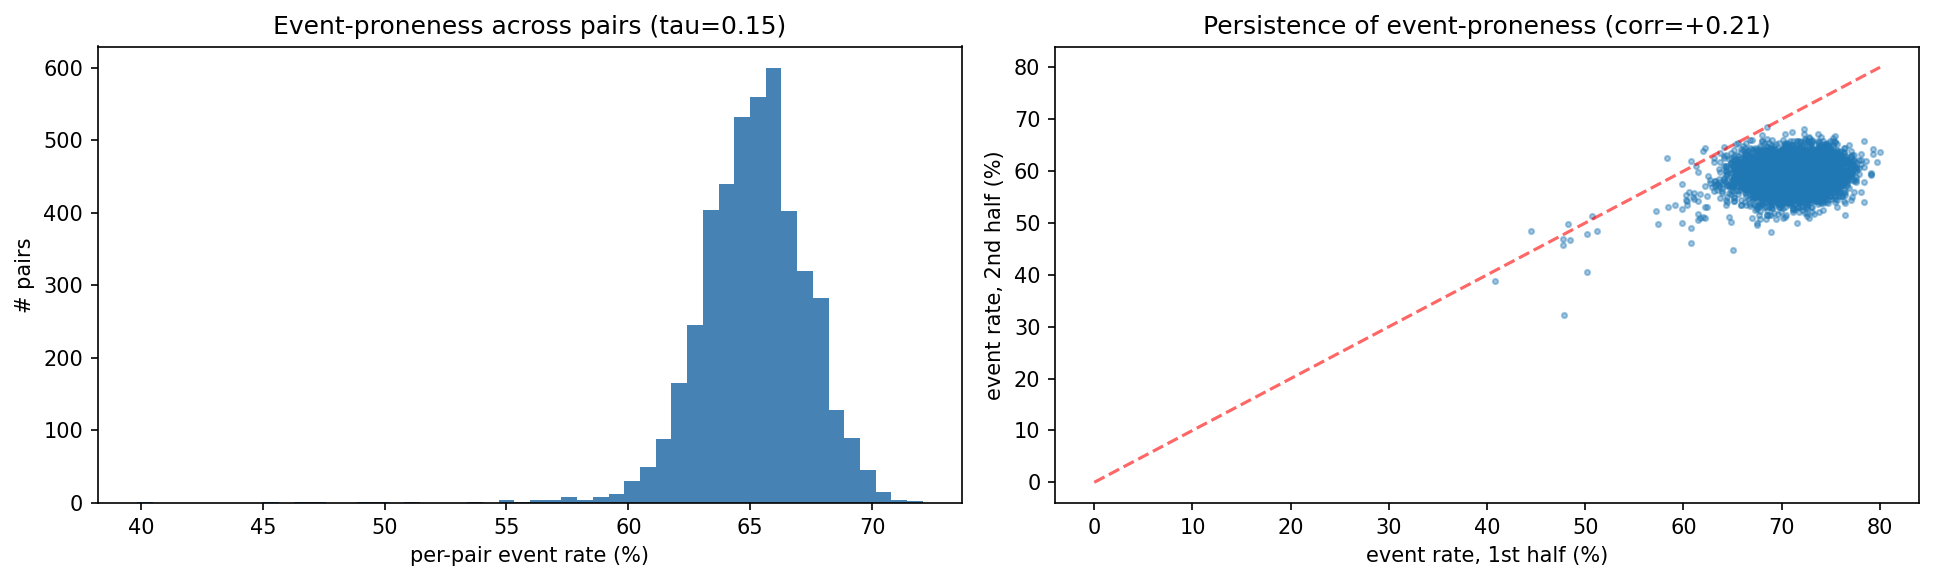
\includegraphics[width=\textwidth]{magnitude_event_structure.png}
\caption{Structure of large coupling changes. Left: distribution of
per-pair large-move frequency, which is concentrated in a narrow band
(no small set of chronically volatile pairs). Right: weak persistence of
per-pair move frequency across the first vs.\ second half of the sample.}
\label{fig:eventstruct}
\end{figure}

\subsection{Selective Prediction: The Model Knows When to Commit}
\label{sec:res_selective}

Because the predictable signal concentrates in large moves, and because
the model's \emph{predicted} change magnitude correlates with the true
magnitude at 0.47, we can recover this skill at inference via selective
prediction (Sec.~\ref{sec:selective}). Table~\ref{tab:selective} sweeps
coverage: emitting predictions only for the most-confident fraction of
cells. Directional accuracy climbs from 73.7\% at full coverage to
85.4\% at 50\% coverage, 91.5\% at 25\%, and 95.6\% at the top decile.
The model thus delivers high-accuracy directional calls precisely on the
relationships it is most confident about --- identified using only
information available at prediction time.

\begin{table}[H]
\caption{Selective prediction: directional accuracy as a function of
coverage, conditioning on the model's own predicted change magnitude.}
\label{tab:selective}
\centering
\begin{tabular}{lcc}
\toprule
\textbf{Strategy} & \textbf{Coverage} & \textbf{Dir.\ Acc.} \\
\midrule
Predict everything (aggregate)      & 100\% & 0.737 \\
Top half by confidence              & 50\%  & 0.854 \\
Top quartile by confidence          & 25\%  & 0.915 \\
Highest-conviction decile           & 10\%  & 0.956 \\
\bottomrule
\end{tabular}
\end{table}

\begin{figure}[H]
\centering
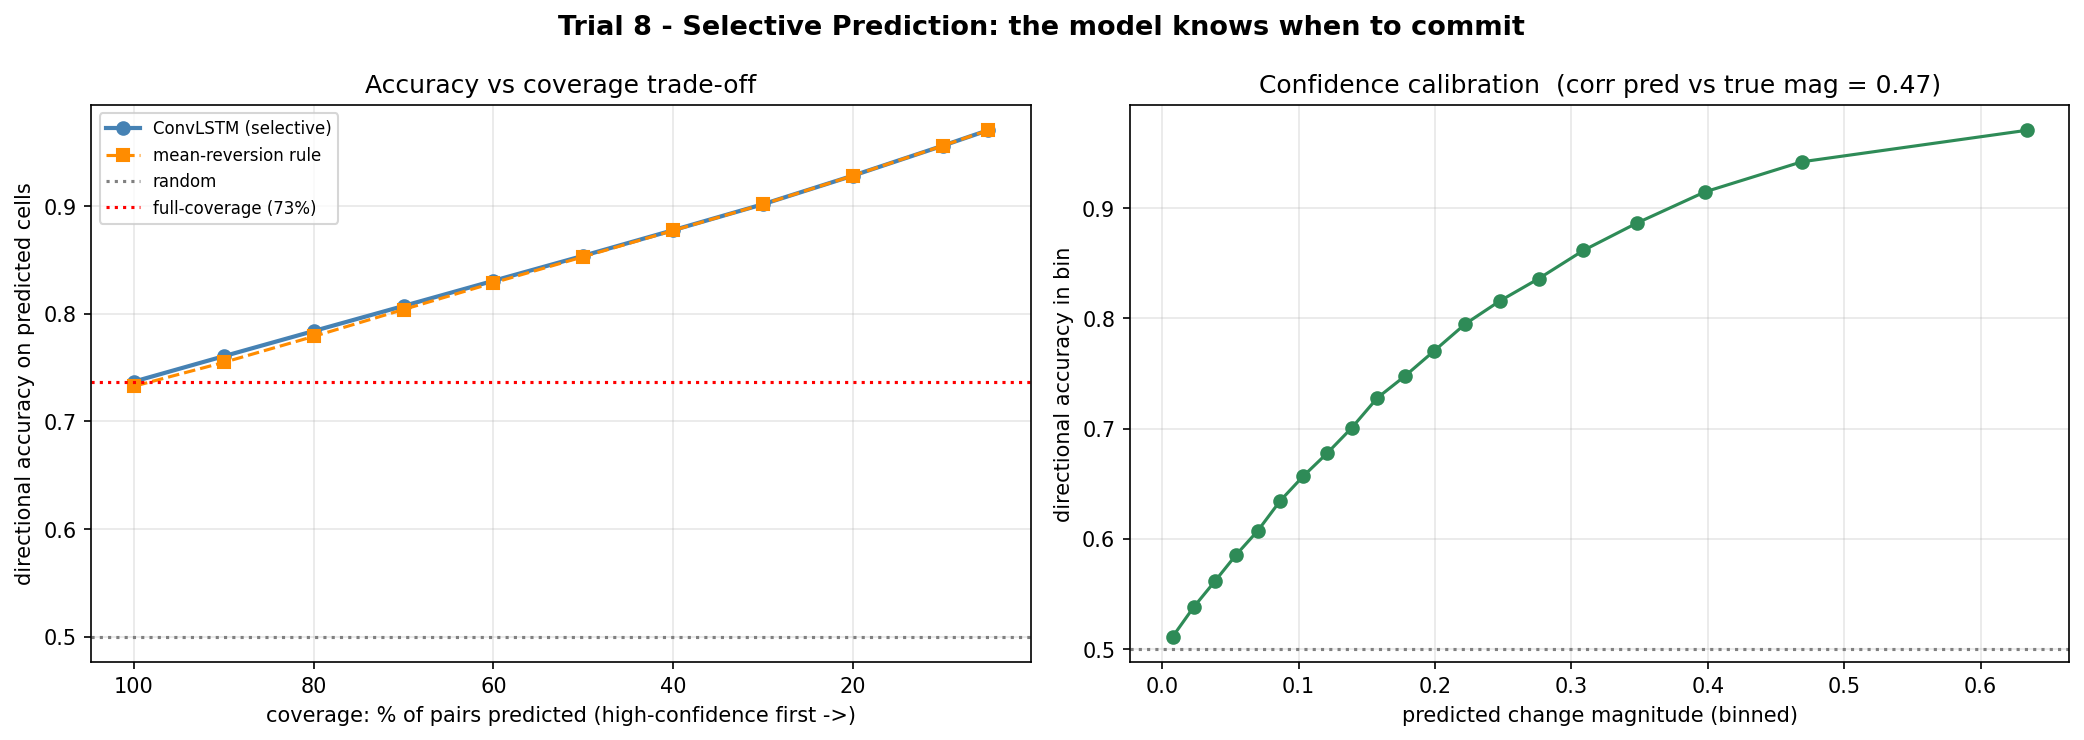
\includegraphics[width=\textwidth]{trial8_selective_prediction.png}
\caption{Selective prediction. Left: directional accuracy versus
coverage (high-confidence cells first); the model far exceeds the
full-coverage 73.7\% as it is allowed to abstain. Right: calibration ---
accuracy increases with the model's predicted change magnitude
(predicted-vs-true magnitude correlation 0.47).}
\label{fig:selective}
\end{figure}

\subsection{External Augmentation is Redundant}
\label{sec:res_external}

Table~\ref{tab:external} summarizes a systematic study of external
signals. India VIX, trained as a second stream in a controlled VIX-on
vs.\ VIX-zeroed comparison, does not improve (and marginally degrades)
the forecast. Diagnostic tests on geopolitical risk (GPR) and
sector-level news sentiment (GDELT) show that global signals --- including geopolitical
risk~\cite{caldara2022measuring} --- carry only a weak leading component
that is redundant with the regime already visible in the matrix (VIX
correlates 0.46 with current average coupling), while granular news tone
from GDELT~\cite{leetaru2013gdelt} carries essentially no leading signal
(pooled partial correlation $0.00$ with sector-coupling change).
The conclusion is consistent across signal types: at this horizon the
predictive content is intrinsic to the coupling structure, and external
augmentation does not extend it.

\begin{table}[H]
\caption{External-signal study. ``Partial lead'' is the partial
correlation with the coupling-change residual after removing
mean-reversion; the model column reports the trained two-stream outcome
where applicable.}
\label{tab:external}
\centering
\begin{tabular}{llc}
\toprule
\textbf{Signal} & \textbf{Type} & \textbf{Outcome} \\
\midrule
India VIX        & global, market-derived   & partial lead $+0.22$; trained model no gain \\
Geopolitical (GPR) & global, exogenous      & partial lead $+0.12$; redundant with VIX \\
News tone (GDELT)  & granular, exogenous    & pooled partial lead $0.00$; no signal \\
\bottomrule
\end{tabular}
\end{table}

Fig.~\ref{fig:vix} shows the controlled two-stream comparison for VIX:
across both aggregate MSE and the full selective-prediction coverage
curve, the VIX-augmented model is statistically indistinguishable from
(and marginally below) the identical VIX-zeroed control.

\begin{figure}[H]
\centering
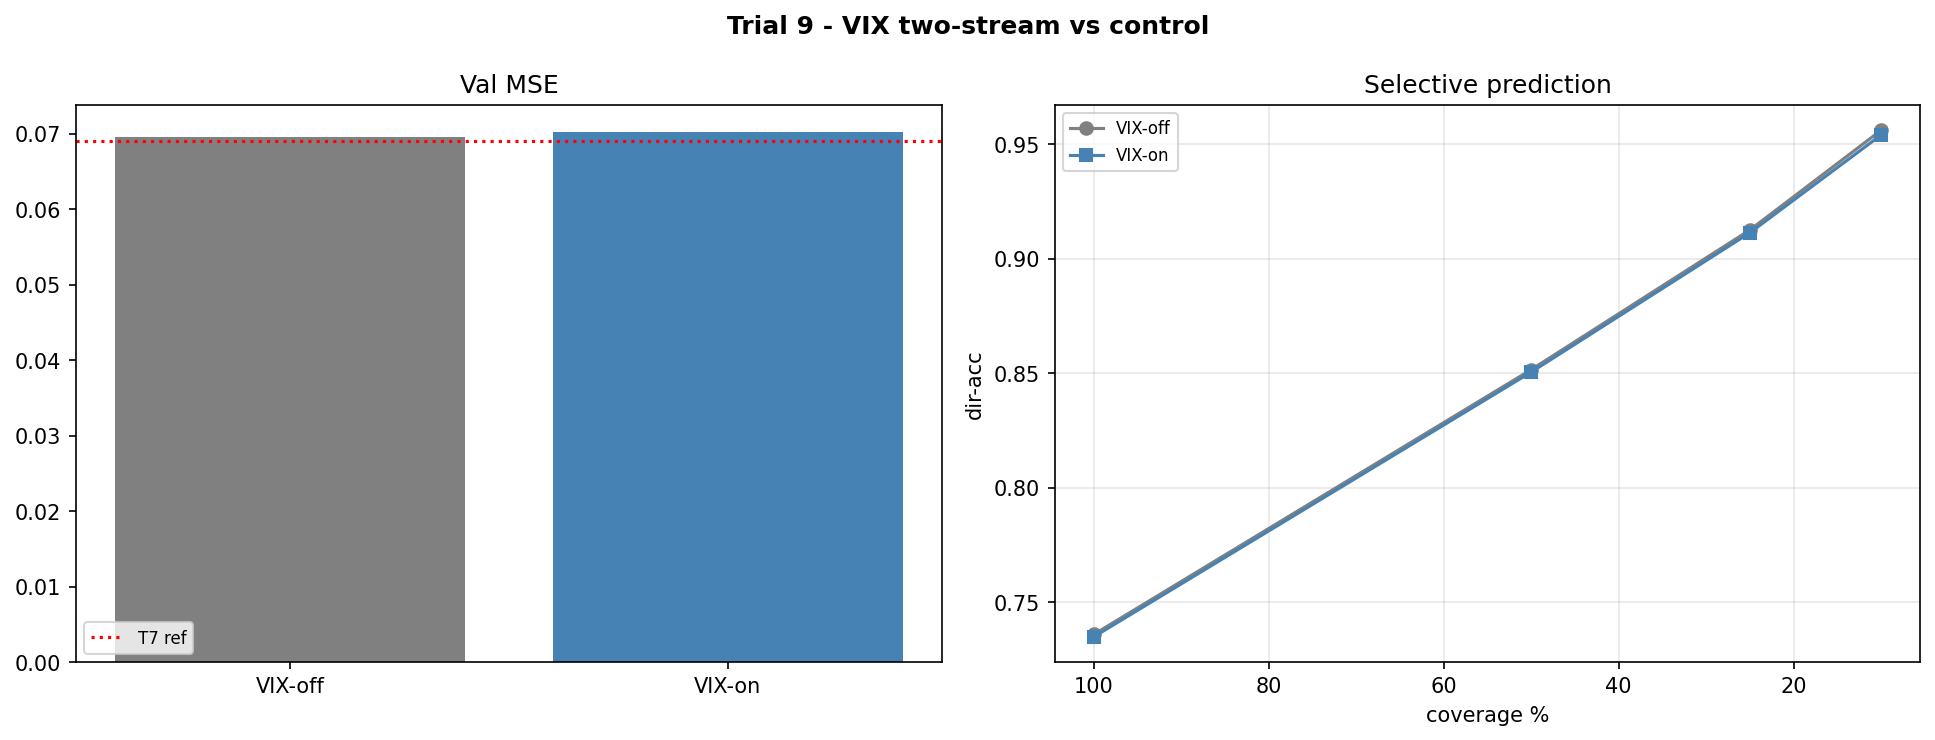
\includegraphics[width=\textwidth]{trial9_vix.png}
\caption{Controlled VIX augmentation. Left: validation MSE, VIX-on
vs.\ the identical VIX-zeroed control. Right: selective-prediction
coverage curves for both. VIX provides no improvement, confirming that
the global volatility regime is already encoded in the matrix.}
\label{fig:vix}
\end{figure}

\subsection{Cross-Stock Inference: A Denoised Covariance}
\label{sec:res_crossstock}

Finally, Table~\ref{tab:crossstock} evaluates the forecast as an
inference tool: predicting one asset's return from a peer's via the
implied regression (Sec.~\ref{sec:crossstock}). Measured by the
correlation between predicted and actual returns, the forecast
(0.283) outperforms persistence (0.188), the historical mean (0.276),
and --- notably --- the realized sample correlation (0.236). The forecast
is thus a \emph{denoised} covariance estimate: smoother and more useful
for inference than the noisy realized correlation. Its advantage over
the static historical mean concentrates on the pairs where it predicts
an unusual relationship (on cells where the forecast's sign disagrees
with the historical norm, it scores 0.57 versus the historical rule's
0.42), consistent with the magnitude finding that the model's value lies
in catching regime changes.

\begin{table}[H]
\caption{Cross-stock inference: correlation between predicted and actual
peer return $r_A$ when inferred from $r_B$ via each correlation estimate.}
\label{tab:crossstock}
\centering
\begin{tabular}{lc}
\toprule
\textbf{Correlation estimate $\rho$} & \textbf{corr(predicted $r_A$, actual $r_A$)} \\
\midrule
Persistence (last observed)     & 0.188 \\
Realized (oracle, true future)  & 0.236 \\
Historical mean                 & 0.276 \\
\textbf{Forecast (ours)}        & \textbf{0.283} \\
\bottomrule
\end{tabular}
\end{table}

% ══════════════════════════════════════════════════════════════════════════════
\section{Discussion}\label{sec:discussion}
% ══════════════════════════════════════════════════════════════════════════════

\subsection{Why the Pair-Level Ceiling Exists: A Structural Argument}

The convergence of all pair-level architectures to $\approx$56\% accuracy,
regardless of model complexity, deserves careful analysis because it
reveals something fundamental about the structure of the prediction
problem rather than about the models themselves.

Consider a pair of stocks $(i, j)$ whose correlation at time $t$ is
$R_t^{(ij)}$. Whether this correlation strengthens or weakens over the
next $H$ bars is determined by two distinct processes: (1) the
\textit{idiosyncratic} relationship between stocks $i$ and $j$ specifically,
and (2) the \textit{market-wide} structural shift that simultaneously
affects many correlations. A pair-level model observing only $R_t^{(ij)}$
cannot distinguish between these two processes. When India VIX spikes and
all correlations rise simultaneously, a pair-level model sees this as
``strengthening'' in the pair's relationship. But the pair has no special
relationship with VIX --- it is simply caught in a market-wide tide.

Formally, let $R_t^{(ij)} = S_t^{(ij)} + \epsilon_t^{(ij)}$ where
$S_t^{(ij)}$ is the systematic component driven by market-wide factors
and $\epsilon_t^{(ij)}$ is the idiosyncratic component. A pair-level
model can observe $R_t^{(ij)}$ but cannot decompose it into $S$ and
$\epsilon$ without observing the full matrix $R_t$. The full matrix
provides the context needed to determine whether the current correlation
level is high relative to the \textit{whole market} (suggesting a
market-wide event) or high only relative to \textit{this specific pair's
history} (suggesting an idiosyncratic change). This is precisely why
the video-based formulation --- which provides the full $N \times N$
matrix as context --- breaks through the ceiling.

\subsection{Why Fiedler Ordering Enables Convolutional Learning}

The Fiedler vector ordering is not merely a visualization technique
--- it is a functional prerequisite for convolutional processing of
the correlation matrix. Without it, convolutional kernels cannot
extract meaningful features because spatially adjacent cells have no
systematic relationship.

To see this concretely: a $3\times3$ kernel applied at position
$(20, 20)$ of a randomly ordered correlation matrix sees the
correlations between three arbitrary, unrelated stocks. The same
kernel applied at the same position of a Fiedler-ordered matrix sees
the correlations within a subgroup of stocks that the spectral
ordering has identified as belonging to the same community. The latter
is a meaningful financial quantity (local cluster cohesion); the
former is noise.

The Fiedler ordering exploits a deep connection between spectral
graph theory and community detection. The Fiedler vector partitions
the graph at the highest-conductance cut --- the partition that
minimizes inter-community edges relative to intra-community edges.
When assets are ordered by Fiedler values, assets with similar Fiedler
values are in the same community (cluster), and their pairwise
correlations appear as a bright block along the diagonal. The
``brightness'' of the block measures community cohesion.

This also explains why the ordering can be computed on the mean
correlation matrix rather than requiring snapshot-by-snapshot
recomputation. The Fiedler ordering provides the \textit{canonical}
arrangement of assets in correlation space --- the stable background
ordering against which temporal fluctuations (blocks brightening or
fading) become legible as a video signal.

\subsection{The 73\% Ceiling is a Diluted Average}

The most important interpretive point of this work is that the
apparent ceiling is an artifact of how directional accuracy is
aggregated. Computed over all $N^2$ cells, the metric averages two
populations: a large majority of near-static pairs whose tiny changes
are dominated by noise, and a minority of pairs undergoing large,
structurally-driven moves. The first population is essentially
unforecastable and pins the average near the mean-reversion rate; the
second is where genuine skill lives (Table~\ref{tab:magnitude}). The
convergence of every architecture and modality to 73\% is therefore not
a failure to extract signal --- it is the signature of an average
dominated by an unforecastable majority. Once predictions are
conditioned on magnitude, the underlying skill (85--96\% on confident
calls) becomes visible. The practical lesson is that correlation
forecasters should be deployed and reported with a coverage axis, not a
single aggregate number.

\subsection{Why Confidence Conditioning Works}

Selective prediction is only useful if the model can identify its own
reliable predictions \emph{ex ante}. It can: the predicted change
magnitude correlates with the realized magnitude at 0.47, so ranking
cells by predicted magnitude approximately ranks them by accuracy. This
calibration arises naturally from the combined loss --- the trajectory
and directional terms encourage the model to commit to a sized change
only when the input dynamics support it, and to predict near-zero change
otherwise. The result is a forecaster that abstains, in effect, on the
pairs where it would otherwise be guessing, and the accuracy--coverage
curve (Fig.~\ref{fig:selective}) quantifies the trade-off a practitioner
can choose along.

\subsection{Why External Signals are Redundant}

That neither market-derived (VIX) nor exogenous (GPR, GDELT) external
signals help is initially surprising but has a clean explanation. Global
risk signals are highly correlated with the \emph{current} level of
average market coupling (VIX correlates 0.46 with it), and that level is
already an input to the model --- it is literally visible in the
correlation frame. A single scalar therefore adds little beyond what the
matrix encodes, and cannot differentially reshape the 4,465 pairwise
relationships. Granular news tone, while genuinely independent of VIX,
carries no measurable leading signal for sector coupling --- consistent
with news being largely priced by the time it is published. The
boundary this establishes is itself a contribution: it locates the
predictive content firmly in the endogenous coupling structure and
its dynamics, not in external context.

\subsection{The Honest Role of Mean-Reversion}

We are deliberate about what the model does and does not add over a
trivial baseline. A one-line rule --- coupling reverts toward its
recent mean --- already attains the 73\% aggregate and rises to 88\% on
large moves, so the bulk of the model's directional skill coincides with
mean-reversion. The deep model's distinctive contributions are narrower
but real: (i) a calibrated confidence signal that enables selective
prediction, and (ii) a denoised covariance estimate that beats the
realized sample correlation for cross-stock inference
(Table~\ref{tab:crossstock}), with its edge over the static mean
concentrated on regime-change pairs. We regard honest delineation of
this boundary as more valuable than an inflated headline number.

Fig.~\ref{fig:horizon} grounds this in the predictability structure of
the data: frame-to-frame coupling changes are strongly mean-reverting
at one step (delta autocorrelation $\approx -0.47$) and decorrelate
almost completely beyond two steps, while the mean-frame baseline MSE is
nearly flat across horizons. The predictable signal is therefore
short-horizon and mean-reversion-dominated --- precisely the regime in
which a calibrated, confidence-aware forecaster is the appropriate tool.

\begin{figure}[H]
\centering
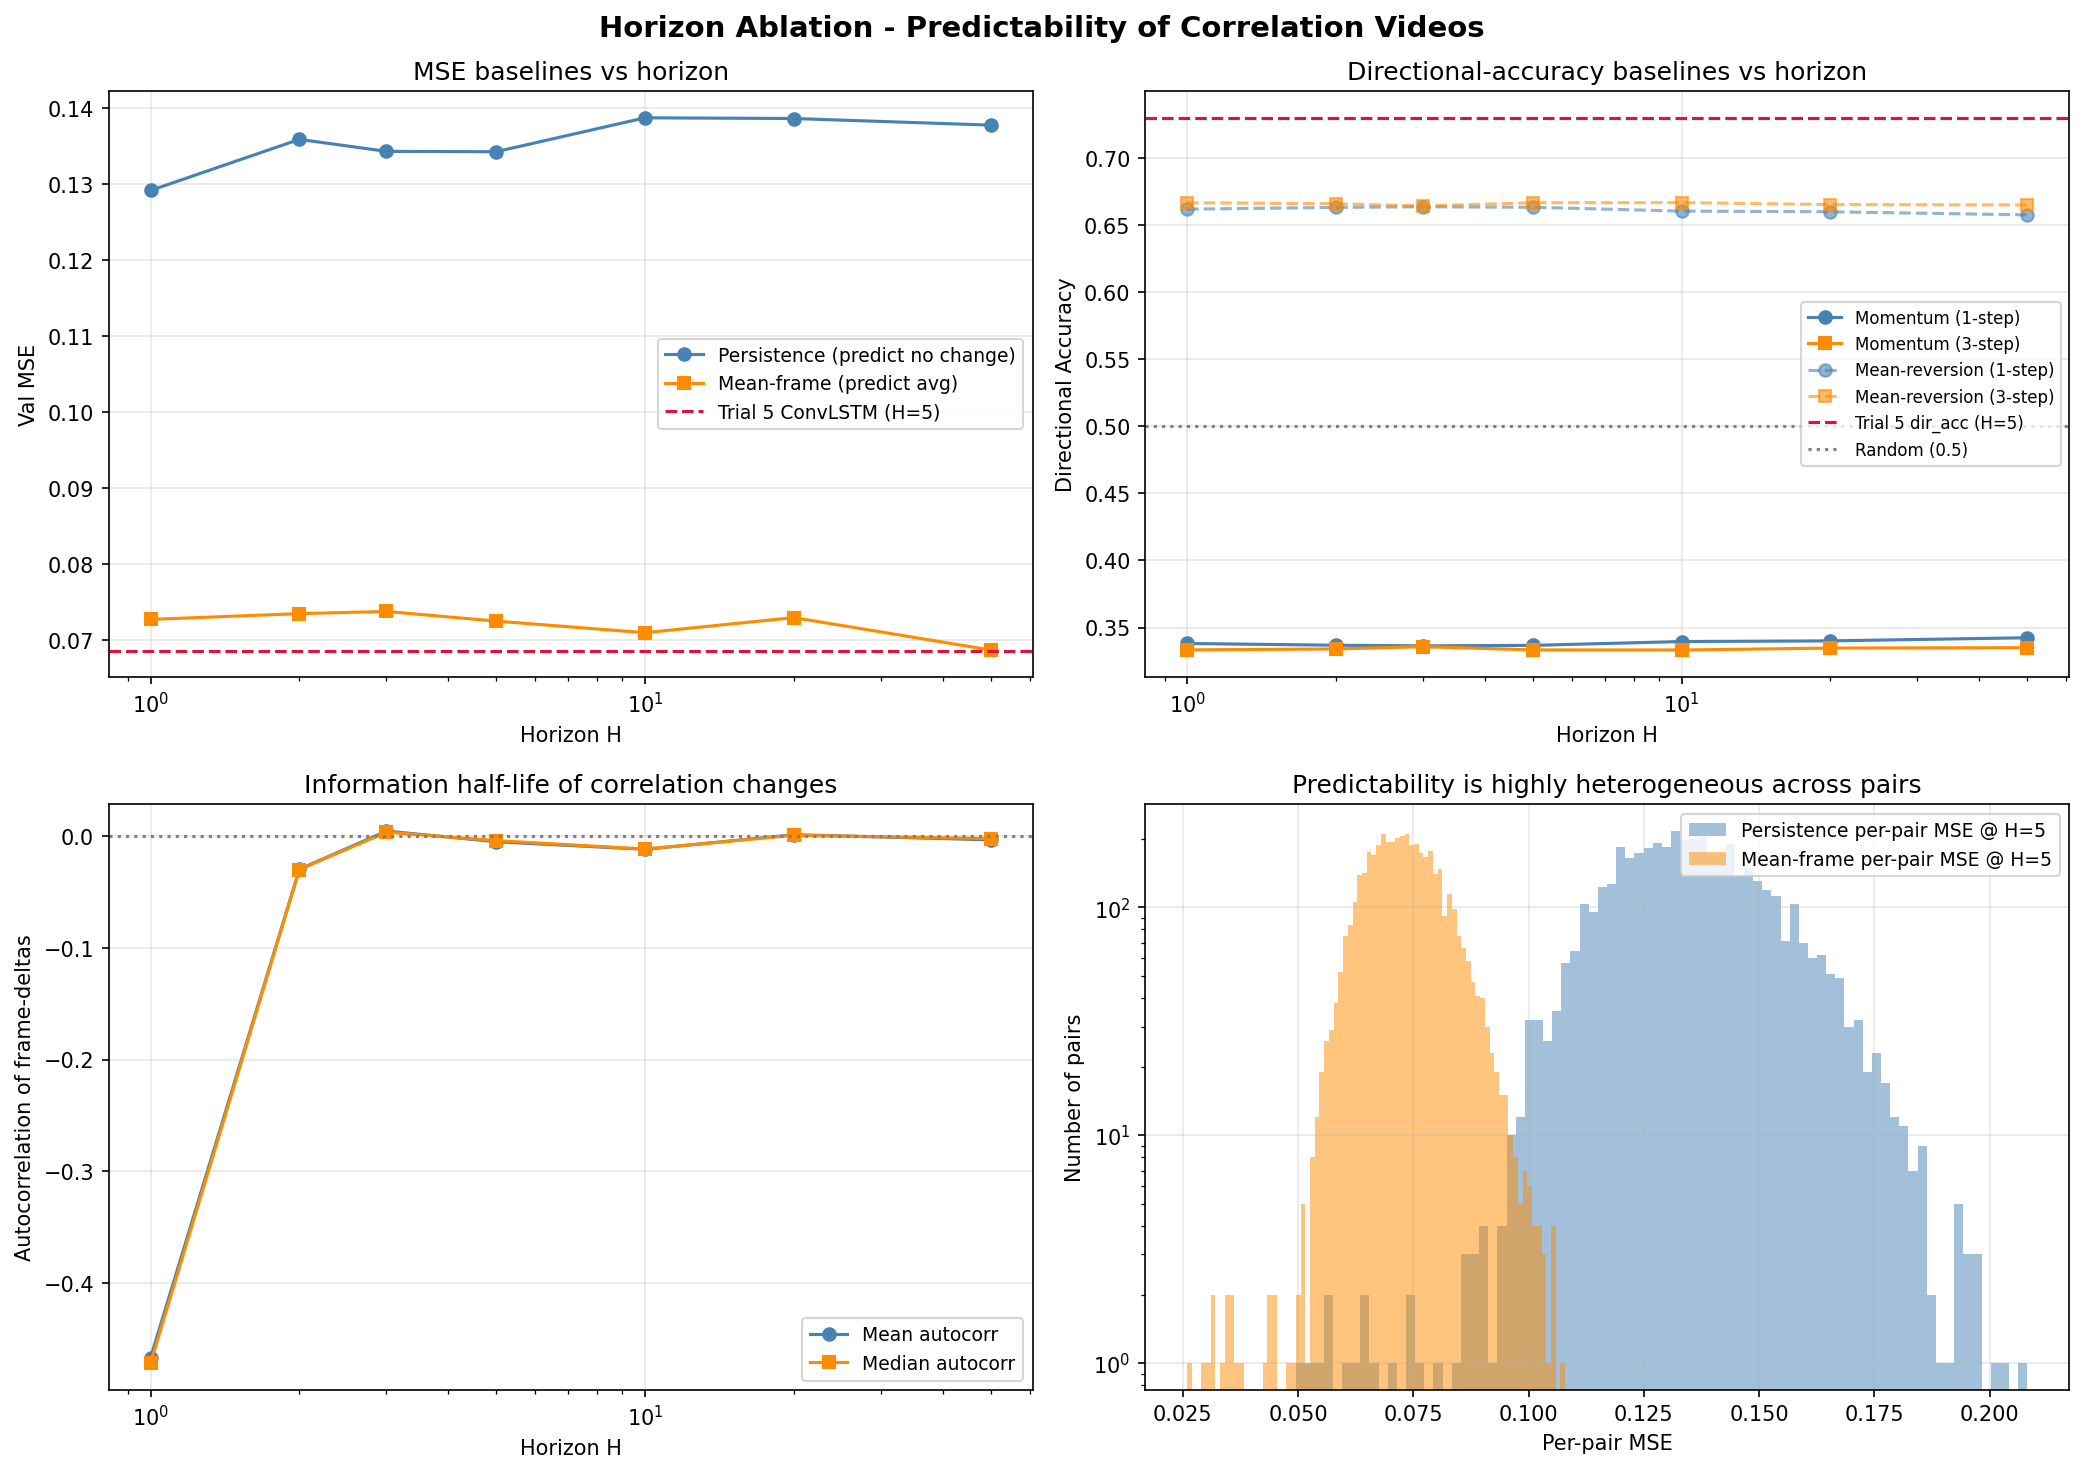
\includegraphics[width=\textwidth]{horizon_ablation.png}
\caption{Predictability structure versus horizon (no training). Baseline
MSE and directional accuracy across horizons, the autocorrelation decay
of frame-to-frame changes, and the heterogeneous per-pair error
distribution. Signal is concentrated at short horizons and dominated by
mean-reversion.}
\label{fig:horizon}
\end{figure}

\subsection{Practical Applications}

The predicted future correlation matrix has several direct applications
in finance, each exploiting a different aspect of the model's output.

\textbf{Diversification monitoring.} Portfolio managers construct
portfolios assuming diversification based on current correlations.
If the model predicts that previously uncorrelated assets will become
highly correlated over the next 5 trading days, the effective
diversification of the portfolio will decrease --- meaning the
portfolio carries more concentrated risk than its current
construction implies. The model enables proactive rebalancing
before the correlation shift materializes, rather than reactive
adjustment after it has already affected portfolio performance.

\textbf{Forward-looking stress testing.} Standard Value-at-Risk
computations use the current covariance matrix. If the model predicts
a regime of elevated correlations (as in the 2022 high-correlation
period), risk managers can compute VaR under the predicted future
correlation structure, providing a forward-looking measure of tail
risk. Under selective deployment, elevated-coupling warnings issued
only at high confidence are correct 85--96\% of the time
(Table~\ref{tab:selective}), rather than the 73\% implied by the
undifferentiated aggregate.

\textbf{Pairs trading signal generation.} Statistical arbitrage
strategies~\cite{avellaneda2010statistical} profit from the convergence
of highly correlated pairs that have temporarily diverged. Selective prediction is a natural fit:
acting only on the model's high-confidence coupling-shift calls yields
directional accuracy in the high 80s to mid 90s, and the
cross-stock-inference result (Sec.~\ref{sec:res_crossstock}) shows the
forecast translates into better estimates of one leg's move given the
other --- directly useful for constructing and hedging the trade.

\textbf{Cluster-based sector rotation.} The predicted future matrix
can be passed to the same Louvain community detection algorithm used
in this work to produce a predicted future cluster structure. Changes
in predicted cluster membership indicate sector rotation: stocks
predicted to leave one cluster and join another are candidates for
momentum-following or mean-reversion trades depending on the
historical behavior of similar transitions.

\subsection{Limitations and Future Directions}

\textbf{Modest edge over mean-reversion.} As emphasized throughout, a
one-line mean-reversion rule attains the same aggregate directional
accuracy as the deep models. The model's value is the calibrated
confidence enabling selective prediction and its role as a denoised
covariance estimate, not a large gain in raw point accuracy. We view
stating this boundary plainly as a strength, but it tempers any claim
of a categorical improvement over simple baselines.

\textbf{EWMA smoothing confound.} The correlation video is built from
EWMA correlations, which are autocorrelated and mean-reverting by
construction. Part of the observed mean-reversion may therefore reflect
the smoothing filter rather than market dynamics. Confirming that the
magnitude and selective-prediction findings persist under raw
windowed-correlation inputs (which we compute but do not analyze here)
is important future work.

\textbf{Single-peer cross-stock inference.} The cross-stock result
infers a return from a \emph{single} peer. Using the full predicted
matrix to infer a stock jointly from all peers --- a factor-style
completion --- should be substantially stronger and is a natural
extension.

\textbf{External data was tested, not omitted.} Unlike many studies, we
explicitly evaluated external augmentation (volume and volatility
correlation, India VIX, geopolitical risk, news sentiment) and found it
redundant at this horizon. The one external avenue we did not exhaust is
granular, scheduled, per-asset information --- notably earnings calendars
--- which (unlike fuzzy news tone) is a hard leading fact and could in
principle reshape specific pairs. Longer/shorter horizons are also open:
our diagnostics indicate the predictable signal concentrates at the
one-step horizon, where the confident-prediction ceiling may be higher.

\textbf{End-to-end portfolio optimization.} The natural economic
validation is to feed the forecast covariance into a minimum-variance
portfolio and measure realized out-of-sample volatility against
sample-covariance and persistence baselines; the cross-stock result
suggests this would be favorable. Connecting the model to a
differentiable portfolio layer and training for a risk-adjusted return
objective directly is a promising direction.

% ══════════════════════════════════════════════════════════════════════════════
\section{Conclusion}\label{sec:conclusion}
% ══════════════════════════════════════════════════════════════════════════════

We formulated correlation matrix forecasting as spatiotemporal video
prediction and, across six architectures and three input modalities,
found a shared $\approx$73\% directional-accuracy ceiling. Our central
result is that this ceiling is a \emph{diluted average}: predictability
rises with the magnitude of the correlation change (to 88\% on the
largest moves), and confidence-conditioned selective prediction recovers
85.4\%, 91.5\%, and 95.6\% directional accuracy at 50\%, 25\%, and 10\%
coverage --- on high-conviction calls the model identifies itself
(predicted-vs-actual magnitude correlation 0.47). The forecast further
acts as a denoised covariance estimate, predicting one asset's move from
a peer's better than persistence, the historical mean, and the realized
sample correlation. A systematic study shows that external regime,
geopolitical, and news signals are redundant with the coupling structure
already encoded in the matrix.

The resulting system is a confidence-aware correlation forecaster whose
practical value lies in knowing \emph{when} to commit: rather than a
single undifferentiated prediction, it offers an accuracy--coverage
trade-off that a risk manager or arbitrageur can choose along. We are
explicit that the bulk of the aggregate directional skill coincides with
mean-reversion; the model's distinctive contributions are calibrated
confidence and denoised cross-stock inference. Future work includes a
formal minimum-variance portfolio backtest, a one-step-horizon study
where the predictable signal is strongest, joint multi-peer inference
from the full predicted matrix, and granular scheduled external signals
such as earnings calendars.

% ── References ────────────────────────────────────────────────────────────────
\begin{thebibliography}{99}

\bibitem{engle2002dynamic}
Engle, R.: Dynamic conditional correlation: A simple class of multivariate
GARCH models. Journal of Business \& Economic Statistics \textbf{20}(3),
339--350 (2002)

\bibitem{ledoit2004honey}
Ledoit, O., Wolf, M.: Honey, I shrunk the sample covariance matrix.
Journal of Portfolio Management \textbf{30}(4), 110--119 (2004)

\bibitem{ledoit2017nonlinear}
Ledoit, O., Wolf, M.: Nonlinear shrinkage of the covariance matrix for
portfolio selection. Review of Financial Studies \textbf{30}(12),
4349--4388 (2017)

\bibitem{bollerslev1990modelling}
Bollerslev, T., Engle, R.F., Wooldridge, J.M.: A capital asset pricing
model with time-varying covariances. Journal of Political Economy
\textbf{96}(1), 116--131 (1988)

\bibitem{chen2018incorporating}
Chen, Y., et al.: Incorporating corporation relationship via graph
convolutional neural networks for stock price prediction. In: Proceedings
of CIKM (2018)

\bibitem{li2021modeling}
Li, W., et al.: Modeling the stock relation with graph network for
overnight stock movement prediction. In: Proceedings of IJCAI (2021)

\bibitem{feng2019temporal}
Feng, F., et al.: Temporal relational ranking for stock prediction.
ACM Transactions on Information Systems \textbf{37}(2), 1--30 (2019)

\bibitem{wu2019graph}
Wu, Z., et al.: Graph WaveNet for deep spatial-temporal graph modeling.
In: Proceedings of IJCAI (2019)

\bibitem{lim2021temporal}
Lim, B., et al.: Temporal fusion transformers for interpretable
multi-horizon time series forecasting. International Journal of
Forecasting \textbf{37}(4), 1748--1764 (2021)

\bibitem{tran2015learning}
Tran, D., et al.: Learning spatiotemporal features with 3D convolutional
networks. In: Proceedings of ICCV (2015)

\bibitem{shi2015convolutional}
Shi, X., et al.: Convolutional LSTM network: A machine learning approach
for precipitation nowcasting. In: Advances in NeurIPS (2015)

\bibitem{tan2019efficientnet}
Tan, M., Le, Q.: EfficientNet: Rethinking model scaling for convolutional
neural networks. In: Proceedings of ICML (2019)

\bibitem{fiedler1973algebraic}
Fiedler, M.: Algebraic connectivity of graphs. Czechoslovak Mathematical
Journal \textbf{23}(2), 298--305 (1973)

\bibitem{mantegni1999hierarchical}
Mantegna, R.N.: Hierarchical structure in financial markets. European
Physical Journal B \textbf{11}(1), 193--197 (1999)

\bibitem{marti2021review}
Marti, G., et al.: A review of two decades of correlations, hierarchies,
networks and clustering in financial markets. Progress in Information
Geometry, 245--274 (2021)

\bibitem{avellaneda2010statistical}
Avellaneda, M., Lee, J.H.: Statistical arbitrage in the US equities
market. Quantitative Finance \textbf{10}(7), 761--782 (2010)

\bibitem{wang2017predrnn}
Wang, Y., Long, M., Wang, J., Gao, Z., Yu, P.S.: PredRNN: Recurrent
neural networks for predictive learning using spatiotemporal LSTMs.
In: Advances in NeurIPS (2017)

\bibitem{bertasius2021space}
Bertasius, G., Wang, H., Torresani, L.: Is space-time attention all you
need for video understanding? In: Proceedings of ICML (2021)

\bibitem{caldara2022measuring}
Caldara, D., Iacoviello, M.: Measuring geopolitical risk. American
Economic Review \textbf{112}(4), 1194--1225 (2022)

\bibitem{leetaru2013gdelt}
Leetaru, K., Schrodt, P.A.: GDELT: Global Data on Events, Location, and
Tone, 1979--2012. In: ISA Annual Convention (2013)

\bibitem{geifman2017selective}
Geifman, Y., El-Yaniv, R.: Selective classification for deep neural
networks. In: Advances in NeurIPS (2017)

\bibitem{bollerslev1986generalized}
Bollerslev, T.: Generalized autoregressive conditional
heteroskedasticity. Journal of Econometrics \textbf{31}(3), 307--327
(1986)

\bibitem{engle1995multivariate}
Engle, R.F., Kroner, K.F.: Multivariate simultaneous generalized ARCH.
Econometric Theory \textbf{11}(1), 122--150 (1995)

\bibitem{andersen2003modeling}
Andersen, T.G., Bollerslev, T., Diebold, F.X., Labys, P.: Modeling and
forecasting realized volatility. Econometrica \textbf{71}(2), 579--625
(2003)

\bibitem{corsi2009simple}
Corsi, F.: A simple approximate long-memory model of realized volatility.
Journal of Financial Econometrics \textbf{7}(2), 174--196 (2009)

\bibitem{laloux1999noise}
Laloux, L., Cizeau, P., Bouchaud, J.P., Potters, M.: Noise dressing of
financial correlation matrices. Physical Review Letters \textbf{83}(7),
1467--1470 (1999)

\bibitem{plerou2002random}
Plerou, V., Gopikrishnan, P., Rosenow, B., Amaral, L.A.N., Guhr, T.,
Stanley, H.E.: Random matrix approach to cross correlations in financial
data. Physical Review E \textbf{65}(6), 066126 (2002)

\bibitem{tumminello2010correlation}
Tumminello, M., Lillo, F., Mantegna, R.N.: Correlation, hierarchies, and
networks in financial markets. Journal of Economic Behavior \&
Organization \textbf{75}(1), 40--58 (2010)

\bibitem{onnela2003dynamics}
Onnela, J.P., Chakraborti, A., Kaski, K., Kert\'esz, J., Kanto, A.:
Dynamics of market correlations. Physical Review E \textbf{68}(5),
056110 (2003)

\bibitem{preis2012quantifying}
Preis, T., Kenett, D.Y., Stanley, H.E., Helbing, D., Ben-Jacob, E.:
Quantifying the behavior of stock correlations under market stress.
Scientific Reports \textbf{2}, 752 (2012)

\bibitem{kim2019hats}
Kim, R., So, C.H., Jeong, M., Lee, S., Kim, J., Kang, J.: HATS: A
hierarchical graph attention network for stock movement prediction.
arXiv:1908.07999 (2019)

\bibitem{sawhney2020deep}
Sawhney, R., Agarwal, S., Wadhwa, A., Shah, R.: Deep attentive learning
for stock movement prediction from social media text and company
correlations. In: Proceedings of EMNLP (2020)

\bibitem{diebold2014network}
Diebold, F.X., Y{\i}lmaz, K.: On the network topology of variance
decompositions: Measuring the connectedness of financial firms. Journal
of Econometrics \textbf{182}(1), 119--134 (2014)

\bibitem{billio2012econometric}
Billio, M., Getmansky, M., Lo, A.W., Pelizzon, L.: Econometric measures
of connectedness and systemic risk in the finance and insurance sectors.
Journal of Financial Economics \textbf{104}(3), 535--559 (2012)

\bibitem{carreira2017quo}
Carreira, J., Zisserman, A.: Quo vadis, action recognition? A new model
and the Kinetics dataset. In: Proceedings of CVPR (2017)

\bibitem{wang2018eidetic}
Wang, Y., Jiang, L., Yang, M.H., Li, L.J., Long, M., Fei-Fei, L.:
Eidetic 3D LSTM: A model for video prediction and beyond. In:
Proceedings of ICLR (2019)

\bibitem{dosovitskiy2021image}
Dosovitskiy, A., et al.: An image is worth 16x16 words: Transformers for
image recognition at scale. In: Proceedings of ICLR (2021)

\bibitem{elyaniv2010foundations}
El-Yaniv, R., Wiener, Y.: On the foundations of noise-free selective
classification. Journal of Machine Learning Research \textbf{11},
1605--1641 (2010)

\bibitem{guo2017calibration}
Guo, C., Pleiss, G., Sun, Y., Weinberger, K.Q.: On calibration of modern
neural networks. In: Proceedings of ICML (2017)

\bibitem{baker2016measuring}
Baker, S.R., Bloom, N., Davis, S.J.: Measuring economic policy
uncertainty. Quarterly Journal of Economics \textbf{131}(4), 1593--1636
(2016)

\bibitem{whaley2009understanding}
Whaley, R.E.: Understanding the VIX. Journal of Portfolio Management
\textbf{35}(3), 98--105 (2009)

\end{thebibliography}

\end{document}